%\documentclass[a4paper]{article}
%\usepackage{ctex}
%\usepackage{amsmath}
%\usepackage{amsthm}
%\usepackage{amssymb}
%%\usepackage{clrscode3e}
%\usepackage{color}
%\usepackage{algorithm}
%\usepackage{algorithmic}
%\usepackage{graphicx}
%%\usepackage{verbatim} %\begin{comment} \end{comment}
%\newtheorem*{theorem}{定理}
%\newtheorem*{definition}{定义}
%\renewcommand{\proofname}{\bf 证明}
%\renewcommand{\figurename}{图}
%\renewcommand{\tablename}{表}
%\renewcommand\qedsymbol{$\blacksquare$}
%\graphicspath{{Problems/}}
%
%\usepackage[top=2cm, bottom=2cm, left=2cm, right=2cm]{geometry}
\chapter{网络流的应用}


%\begin{document}
   % \maketitle
    \section{上节回顾}
        \paragraph{}上一节我们讲到了网络流, 以及计算网络流的很多种算法, 包括最原始的Ford-Furkerson, 后面的Edmonds-Karp算法, Dinitz算法, 以及Tarjan在1983年提出的Push-Relabel算法. 其中有一个很关键的技巧就是缩放(scaling). 
    \section{本节提要}
        \paragraph{}本节我们要讲网络流的应用. 因为网络流和线性规划是非常强有力的武器, 掌握了他们之后, 一大类的问题都可以归结成这种技术. 在这里提醒大家一点, 建模的本领是我们的看家本领之一, 而建模的本事在以下几个地方特别需要强调: 
        \begin{enumerate}
        \item 线性规划, 还有我们后面要讲的半正定规划
        \item 网络流, 也就是本节的主题
        \item 问题的规约, 下节课我们将NP-hard的时候将会提到
        \end{enumerate}
        \paragraph{}本节要将以下几个部分:
        \begin{itemize}
        \item 扩展的最大流问题: 无向图上的最大流; 多源点、多汇点的流通问题;  每条边有流量下界的流通问题; 最小费用流{\sc Minimum Cost Flow};
        \item 使用网络流和原始对偶技术解决实际问题:
            \begin{enumerate}
            \item 集合划分: 给我们一个集合, 让我们把集合分成两堆, 有可能可以建模成网络流, 常见的问题有:{\sc ImageSegmentation}, {\sc ProjectSelection}, {\sc ProteinDomainParsing};
            \item 在网络中寻找路径: 常见的有这些问题: {\sc FlightScheduling}, {\sc Disjoint Paths}, {\sc BaseballElimination};
            \item 拆分数字: {\sc BaseballElimination};
\item 构造匹配: {\sc BipartiteMatching}, {\sc SurveyDesign};
            \end{enumerate}
        \item 匹配的扩展: 这是计算机算法历史上十分重要的一个部分,比如二分图匹配{\sc BipartiteMatching}, 加权二分图匹配{\sc WeightedBipartiteMatching}, 一般图匹配{\sc GeneralGraphMatching}, 加权一般图匹配{\sc WeightedGeneralGraphMatching};
        \item 网络流发展的简要历史.
        \end{itemize}
    \section{网络流问题的扩展}
        \paragraph{}网络流问题有以下几个扩展:
        \begin{enumerate}
        \item 无向图上的最大流({\sc MaximumFlow})问题: 
        \item 多源点、多汇点的流通({\sc Circulation})问题;  
        \item 每条边有流量下界的流通({\sc Circulation})问题; 
        \item 最小费用流问题({\sc Minimum Cost Flow});
        \end{enumerate}
    \subsection{无向图上的最大流问题}
        \subsubsection*{问题的定义}
        \paragraph{}一个无向图上的最大流问题可以形式化定义如下:
        \paragraph{输入:}  一个 {\bf 无向图}  $G=<V, E>$, 每条边$e$有容量$C(e) > 0$. 两个特殊的节点: {\bf 源点 $s$} 和 {\bf 汇点 $t$}; 
\paragraph{输出:} 对每条边 $e$, 指定一个流量值 $f(e)$, 使得总的流量值 $\sum_{e=(s,v)} f(e)$最大.
        \paragraph{流性质:} 只有这里和之前讲的有向图上的最大流问题不同
        \begin{enumerate}
        \item{容量限制:}  从$u$到$v$和从$v$到$u$的流量加起来不能超过$(u, v)$上的容量, 即{\bf $0 \leq f(u, v) + f(v, u) \leq C(u, v)$},  $\forall(u,v) \in E$;
        \item{存储(Conservation)限制:}  $f^{in} (v) = f^{out} (v)$,  $\forall v\in V \backslash\{s, t\}$.
        \end{enumerate}
        \subsubsection*{一个例子}
        \paragraph{}下面我们举一个例子:
        \begin{figure}[h]
            \center
            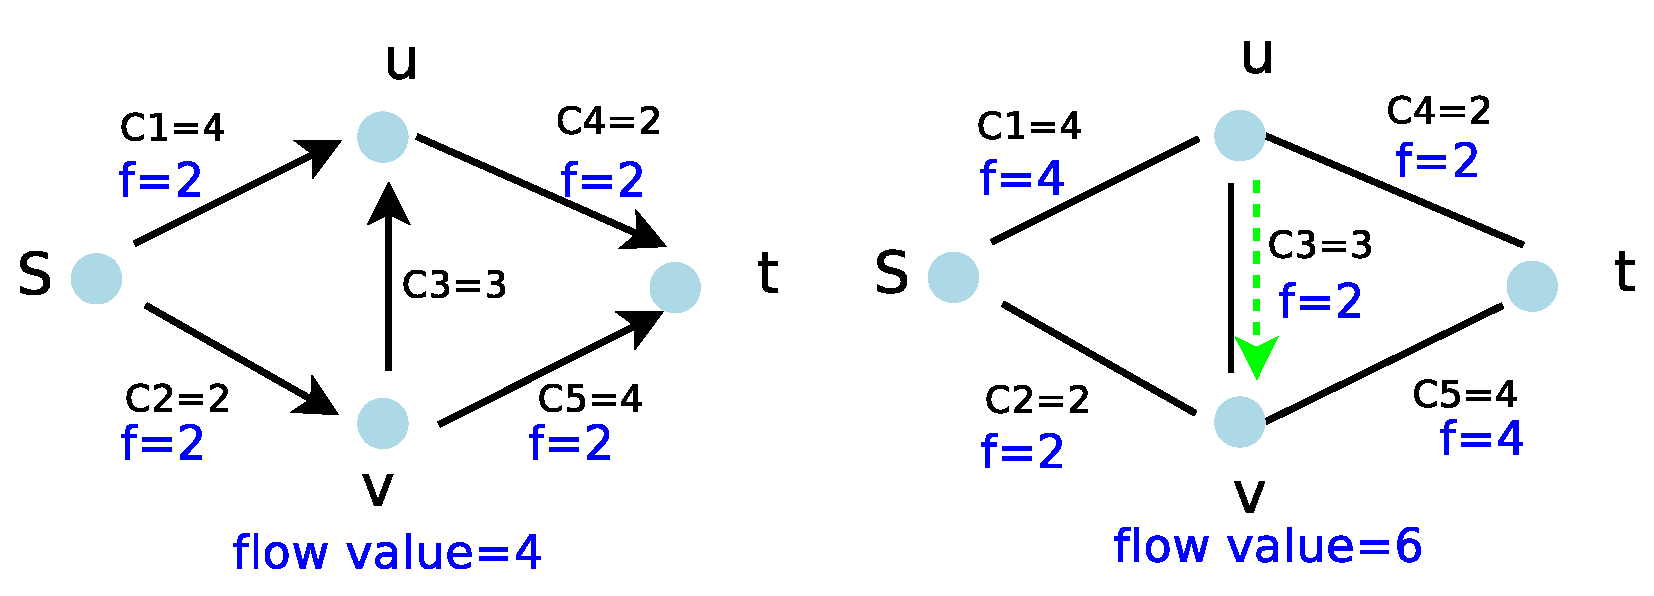
\includegraphics[width=3.3in] {L10-networkflowundirectedexample.eps}
            \caption{有向图与无向图上的最大流}
            \label{Figure: directed_and_undirected_maximum_flow}
        \end{figure}
        \paragraph{}如\figurename\ref{Figure: directed_and_undirected_maximum_flow}所示, 左边是上一节我们遇到的有向图上的最大流, 使用上一节的方法, 可以得到总流量是4. 而右边是一个无向图, 比如$s$到$u$, 可以看做是一个双向的铁路, 可以从$u$往$s$运, 也可以从$s$往$u$运, 它们加起来不能超过4吨. 这是一个很自然的改变, 我们也经常遇到. 这时在使用上一节讲到的那些算法就会出问题了, 如\figurename\ref{Figure: directed_and_undirected_maximum_flow}右边的所示, 可以运6吨. 也就是说我们上一节的算法不能直接使用, 需要做一些修改.
        \subsubsection*{算法}
        \paragraph{}那么, 有向图我们会做了, 无向图不会做. 我们能不能将无向图转换成有向图? 首先, 将无向图转换成有向图, 在我们会做的有向图上面做完之后, 再把它改一下, 回归到原始的问题. 这种思想在后面两个问题中也将用到. 算法大意如下:
        \paragraph{} 无向图$G$上的最大流算法
  \begin{algorithmic}[1]
    \STATE 将无向图$G$转换成有向图$G'$;
    \STATE 使用Ford-Fulkerson算法计算$G'$上的最大流;
    \STATE 校正(revising)每条边上的流量, 使其满足无向图上的流量限制;
  \end{algorithmic}

        \paragraph{}大意明白了, 接下来我们一步一步具体看, 首先将无向图$G$转换成有向图$G'$:
		\begin{enumerate}
		\item 添加边:  对图$G$中每一条边$(u,v)$, 在$G'$中引入两条新的边$e=(u,v)$和$e'=(v,u)$;
		\item 设置容量: $C(e')=C(e)=C(u,v)$.
		\end{enumerate}
		\begin{figure}[h]
		    \centering
			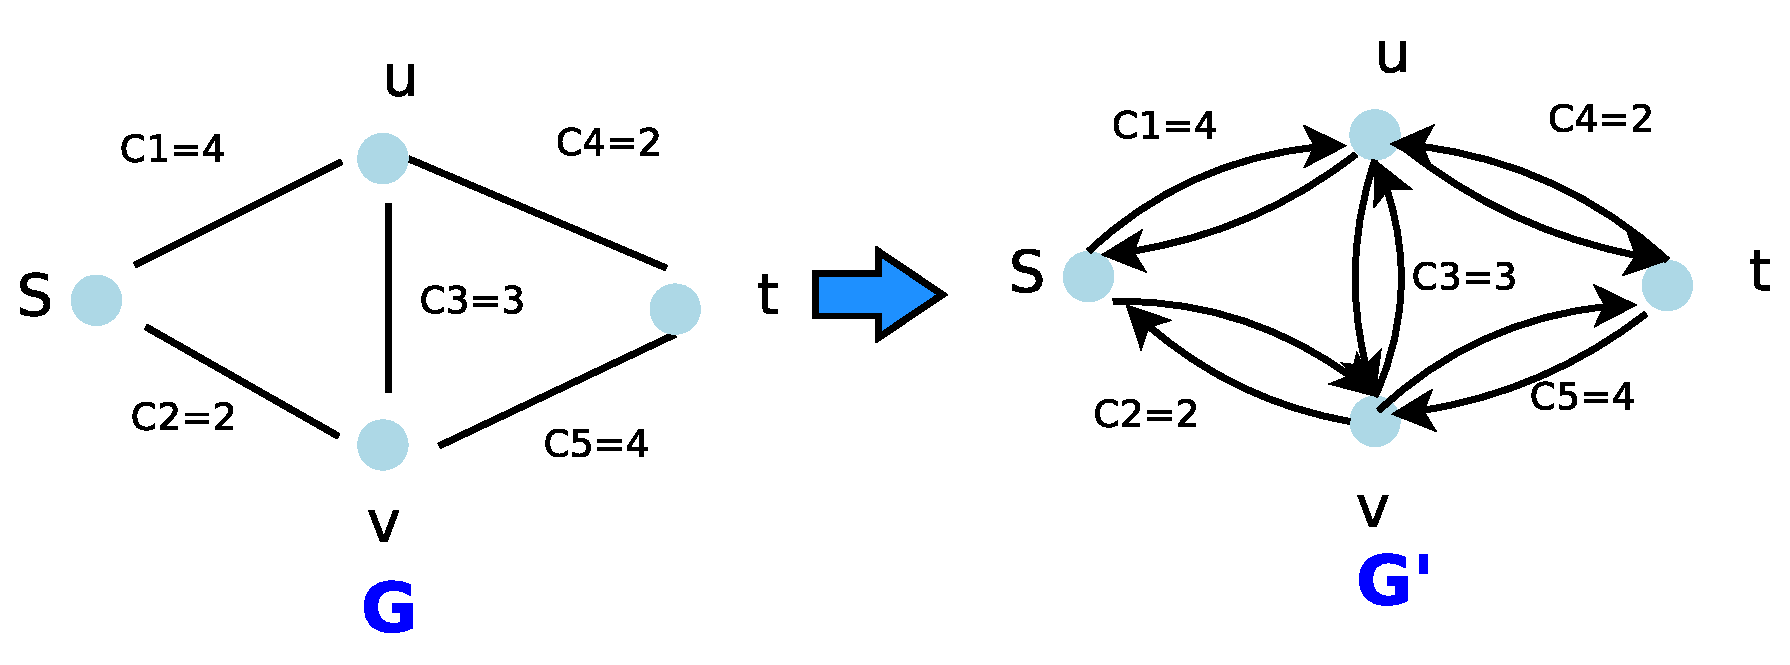
\includegraphics[width=3.6in] {L10-networkflowundirecteddirected.eps}
			\caption{无向图到有向图的转换}
		\end{figure}
		\paragraph{}接下来, 在$G'$上使用有向图的最大流算法, 得到如\figurename\ref{Figure: directed_flow_in_undirected_graph}上蓝色的边所示的一个最大流. 唯一的问题是在边$(u,v)$上, 从$u$到$v$运$3$吨, 从$v$到$u$运$1$吨,总共加起来是$4$吨, 超过了原图$G$中的容量限制$3$.
		\begin{figure}[h]
		    \centering
            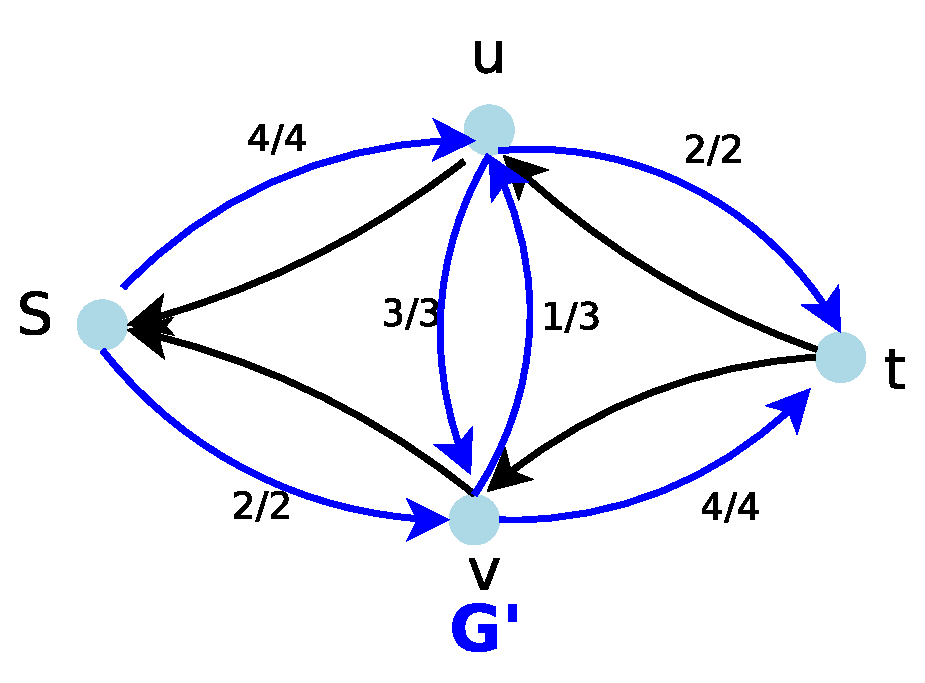
\includegraphics[width=1.5in] {L10-networkflowundirecteddirectedflow.eps}
            \caption{$G'$上的一个最大流}
            \label{Figure: directed_flow_in_undirected_graph}
        \end{figure}
        \paragraph{}最后, 校正每条边上的流量, 已消除像$(u,v)$边上这样违反容量限制的问题. 如\figurename\ref{Figure: revising_in_undirected_graph}所示, 只要有$u-v$这样的一个圈, 那么从$v$到$u$就不运送了, 而从$u$到$v$少运$1$吨, 运$2$吨就可以了, 其他的边没有变化. 简单来说, 双向铁路上流量小的边就不运了, 而流量大的边的流量减少相同的值. 形式化的, 两条边$e=(u,v)$和$e'=(v,u)$, 如果有$f(e)=a>b=f(e')$, 则设定$f(e)=a-b$且$f(e')=0$
        \begin{figure}[h]
            \centering
            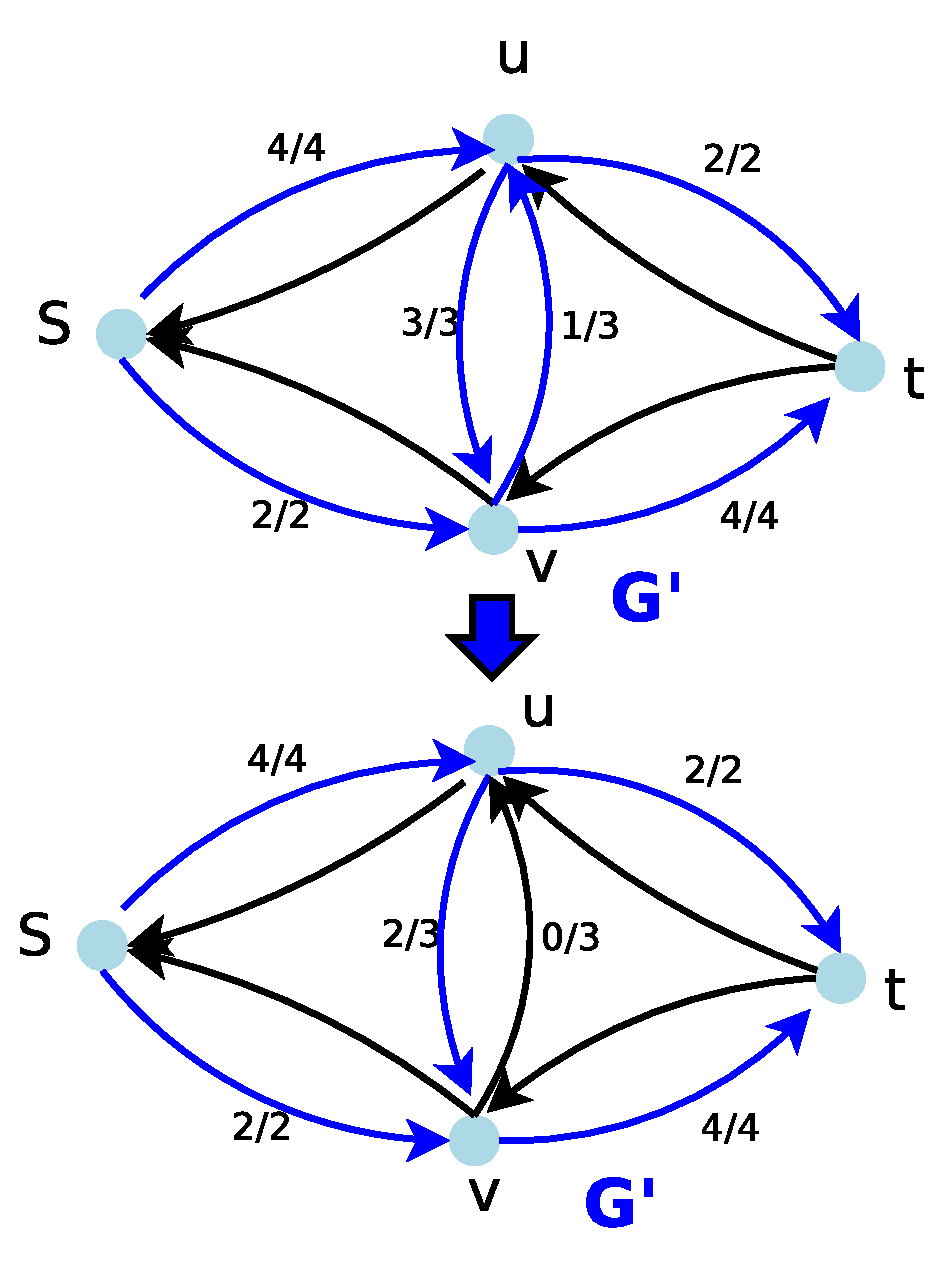
\includegraphics[width=1.8in] {L10-networkflowundirecteddirectedflowrevising.eps}
            \caption{校正每条边上的流量}
            \label{Figure: revising_in_undirected_graph}
        \end{figure}
        \subsubsection*{算法的正确性}
        \paragraph{}由此, 我们可以得到如下的定理:
        \begin{theorem}
        在有向图$G$上存在一个最大流$f$, 使得$f(u,v) = 0$或$f(v,u) = 0$. 
        \end{theorem}
        \paragraph{}这么改之后我们要验证两个条件. 第一, 每个城市是不是流入等于流出; 第二, 每条边上的运量之和不超过边上的容量. 第一个是很显然的. 第二个, 我们有$f(u,v) \leq C$且$f(v,u) \leq C$, 假设$f(v,u) \leq f(u,v)$, 我们有$f'(u,v) = f(u,v) - f(v,u) \leq C$, 满足容量条件, 如\figurename\ref{Figure: revising_on_u_v}所示. 
        \begin{figure}[h]
            \centering
            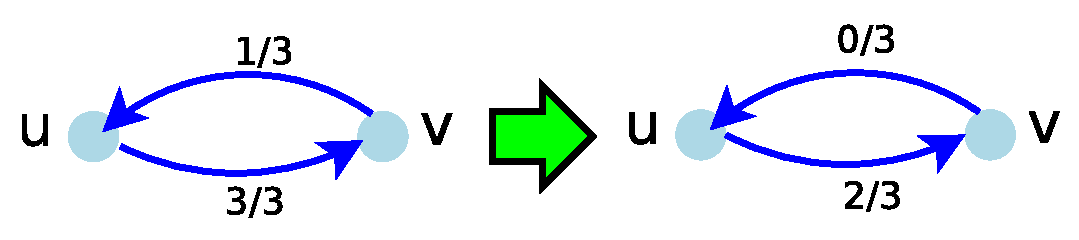
\includegraphics[width=1.9in] {L10-networkflowrevising.eps}
            \caption{对$(u,v)$边进行流量校正}
            \label{Figure: revising_on_u_v}
        \end{figure}
		\begin{proof}
		\item 假设$f'$是有向图$G'$上一个的最大流, 满足$f'(u,v) > 0$且$f'(v,u) > 0$. 我们将流$f'$转换成无向图上的最大流$f$如下:
		\item 令$\delta=\min\{ f'(u,v), f'(v,u) \}$.
		\item 令$f(u,v) = f'(u,v) - \delta$, 令$f(v,u) = f'(v,u) - \delta$. 我们有$f(u,v) = 0$或者$f(v,u)=0$.
		\item 显然这样定义的无向图上的流量满足容量限制和存储限制.
		\item $f$的值和$f'$相同, 所以$f$是最优的.
		\end{proof}
	
	
	\subsection{多源点、多汇点的流通问题}
	    \subsubsection{问题的定义}
	    \paragraph{}一个多源点、多汇点的流通问题可以形式化定义如下:
        \paragraph{输入:}一个图$G=<V, E>$, 每条边$e$有容量$C(e) > 0$. 存在多个源点$s_i$和多个汇点$t_j$. 每个汇点$t_j$都有一个需求$d_j > 0$, 每个源点$s_i$可以提供$d_i$(表示为负的需求$d_i < 0$).
        \paragraph{输出:}一个{\bf 可行流通(feasible circulation)} $f$, 它满足所有节点的要求, 也就是:
        %我这里翻译上不是很确切 to satisfy all demand requirements using the available supply, i.e.,
        \begin{enumerate}
        \item{容量限制:}  $0 \leq f(e) \leq C(e)$;
        \item{需求限制:}  $f^{in} (v) - f^{out} (v) = d_v$;
        \end{enumerate}
	    \paragraph{}为表述简单, 我们使用一个小技巧, 对所有既不是源点也不是汇点的节点$v$, 我们定义$d_v=0$. 由此, 我们有$\sum_i d_i = 0$. 同时我们令$D=\sum_{d_v >0 } d_v$为{\bf 总需求量}.
	    \paragraph{}注意, 流通{\sc Circulation}问题和多物品流{\sc MultiCommodities}问题是不同的: 
        \begin{enumerate}
        \item  {\sc 流通}问题: 流网络中只存在一种货物. 一个汇点$t_{i}$可以从{\bf 任意一个}源点接受货物. 也就是说, 汇点$t_{i}$的需求是由所有源点来的货物组合而来.
        \item {\sc 多物品流}问题: 流网络中有多种物品. 比方说, 在我们需要在同一个网络中运送食物和石油. 汇点$t_i$(假设需要食物)只接受从$s_i$(假设供应食物)运出的货物$k_i$. 两种货物共享这个网路. 到目前为止, 现行规划是解决多物品流的唯一的多项式时间算法.
        \end{enumerate}
	    \paragraph{}我们来看一个例子, 如\figurename\ref{Figure: multi_s_and_t_circulation_example}所示. $s_1, s_2$都是货源地, 都想往外运$3$吨货物, $t_1$需要$2$吨货物, $t_2$需要$4$货物, 问题就是我们该怎么运?
	    \begin{figure}[h]
	        \centering
            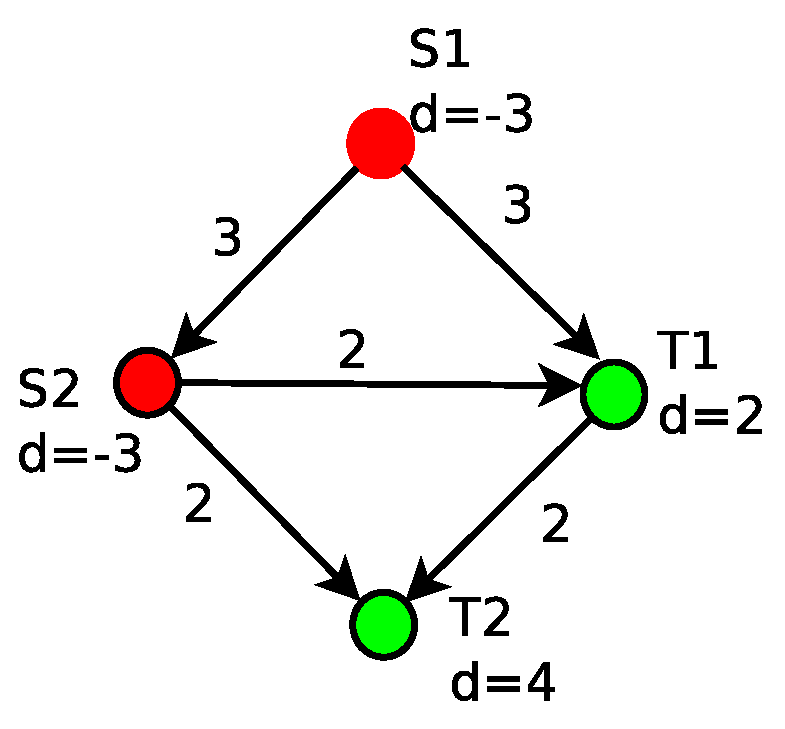
\includegraphics[width=1.3in] {L10-circulationexample.eps}
            \caption{两个源点$s_1, s_2$和两个汇点$t_1, t_2$的流通问题}
            \label{Figure: multi_s_and_t_circulation_example}
        \end{figure}
        
        \subsubsection*{算法}
        \paragraph{}现在我们来解这个问题. 再回到原初的想法, 给我们一个问题, 我们首先考虑这个问题能不能分解, 对这个问题, 可以分. 比如, 从$s_1$向$s_2$运$3$吨, 然后再把这条边删掉. 但是这个分法会引来很多麻烦, 子问题的数目可能非常多. 所以我们就先不分, 考虑改进(improvement)的做法. 
        \paragraph{}其实, 使用改进的做法, 就算没有下面的算法, 我们也可以使用之前所学的一个强力的武器—线性规划来解这个问题. 我们很容易把它写成线性规划, 写完之后, 如果不怕麻烦的话就机械性的把这个问题的原始对偶以及DRP写出来, 这个问题就求解了. 事实上, 我们接下来将的方法都可以通过原始对偶推出来, 只不过是它的一个简化的实现罢了.   
        \paragraph{}那么我们首先先把这个问题写成线性规划, 对每条边$(u,v)$定义一个变量$f(u,v)$表示这条边上的流. 由边上有容量限制和节点的需求限制, 可以得到如下的线性规划表达式(由于只要求可行解, 目标函数为0):
        \begin{equation*}
\begin{array}{cl@{}ll}
\text{Min}  & 0 &\\
\text{s.t.} & f(u,v) \leq C(u,v),\;  & \forall (u,v) \in E  \\
            & \sum_{v}{f(v,u)} - \sum_{v}{f(u,v)} = d_u, \;  & \forall u \in V \\
            & f(v,u) \geq 0, \; & \forall (u,v) \in E \\
            
\end{array}
        \end{equation*}
        
        \paragraph{}接下来, 我们考虑更加简单的做法. 老样子, 这里有多个收货地, 我们过去做的只有单个发货收货地. 跟之前一样, 能不能把这个不会做的问题转化成会做的问题呢? 我们构造一个图, 这个图上只有一个发货地, 一个收货地, 然后做网络流, 最后在返回到原始问题. 就是如下的做法:
        \begin{algorithmic}[1]
            \STATE 对原网络增加一个超级源点$S^*$和超级汇点$T^*$, 构成一个扩展网络$G'$;
            \STATE 使用Ford-Fulkerson算法计算得到$G'$上的一个最大流$f$;
            \STATE 如果最大流的值等于$D=\sum_{v: d_v > 0} d_v$, 则返回流$f$.
        \end{algorithmic}
        \paragraph{}接下来, 我们一步一步来看.
        \subsubsection*{第一步: 构造扩展网络$G'$}
        \paragraph{}{\bf 转化:} 如\figurename\ref{Figure: circulation_constructing_ampled_network}所示, 构造网络$G'$: 增加一个超级源点$s^*$, 指向所有的货源地$s_i$, 链接的边上的容量为$C(s^*,s_i)=-d_i$. 类似的, 增加的一个超级汇点$t^*$, 所有汇点$t_j$都指向它, 对应边上权值为$C(t_j,t^*)=d_j$.
        \begin{figure}[h]
            \centering
            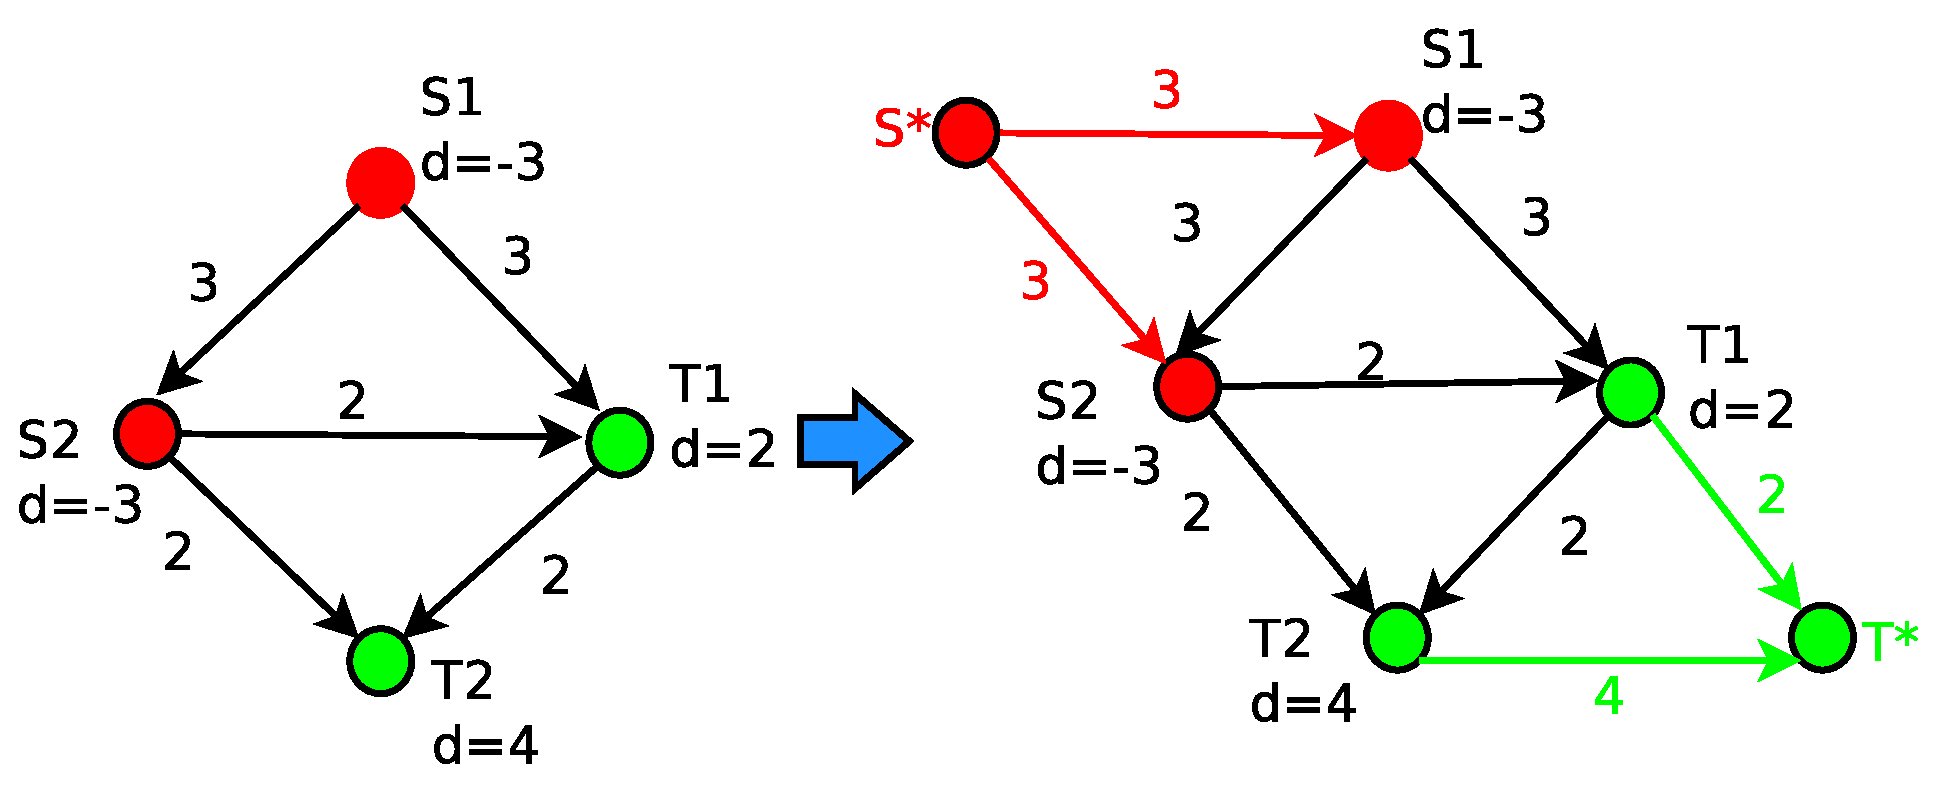
\includegraphics[width=3.5in] {L10-circulationexamplenetwork.eps}
            \caption{构造扩展网络$G'$}
            \label{Figure: circulation_constructing_ampled_network}
        \end{figure}
        \paragraph{}这种转化方法我们可以这样看: 比如$s_1$, 有$3$吨货要往外运, 我们就假设这$3$吨货是从$s^*$运来的. 同理, 对收货地$t_1$和$t_2$最终也要运到$t^*$.
        \subsubsection*{第二步: 计算$G'$上的最大流}
        \paragraph{}接下来, 问题就转化成我们会做的问题了, 在$G'$上跑Ford-Fulkerson, 得到最大流如\figurename\ref{Figure: circulation_maximum_flow}所示.
        \begin{figure}[h]
            \centering
            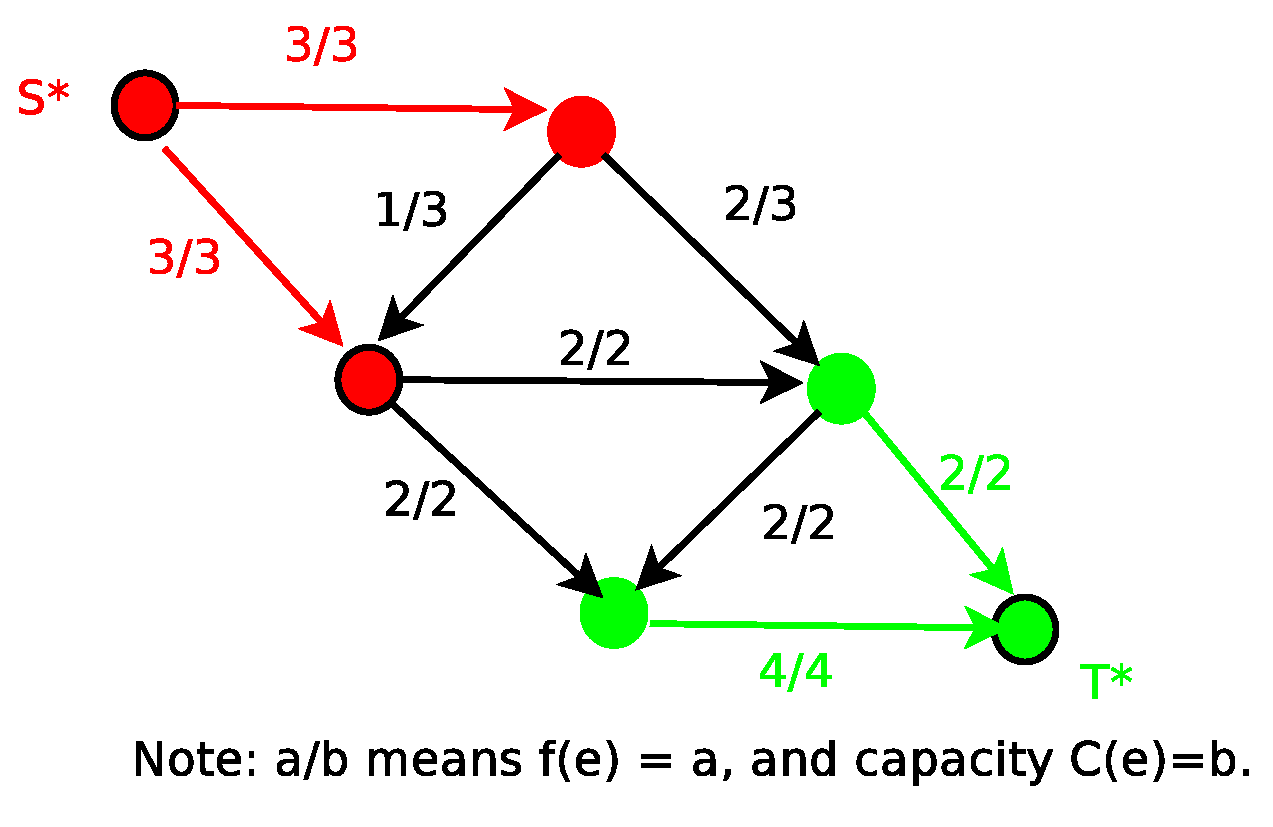
\includegraphics[width=3in] {L10-circulationtomaximumflow.eps}
            \caption{计算$G'$上的最大流}
            \label{Figure: circulation_maximum_flow}
        \end{figure}
        \subsubsection*{第三步: 检查$G'$上的最大流}
        \paragraph{}如\figurename\ref{Figure: circulation_maximum_flow_checking}所示, 我们得到的最大流是$6$吨, 等于$S^*$运出货物的总量, 即$6 = \sum_{v, d_{v}>0} d_{v}$. 因此,原始问题是有解. 只要把边原封不动地拷过去就得到了一个原始流通问题的可行解. 但是如果求得的最大流不是$6$, 那就意味着原问题没有一种可能的流通方案
        \begin{figure}[h]
            \centering
            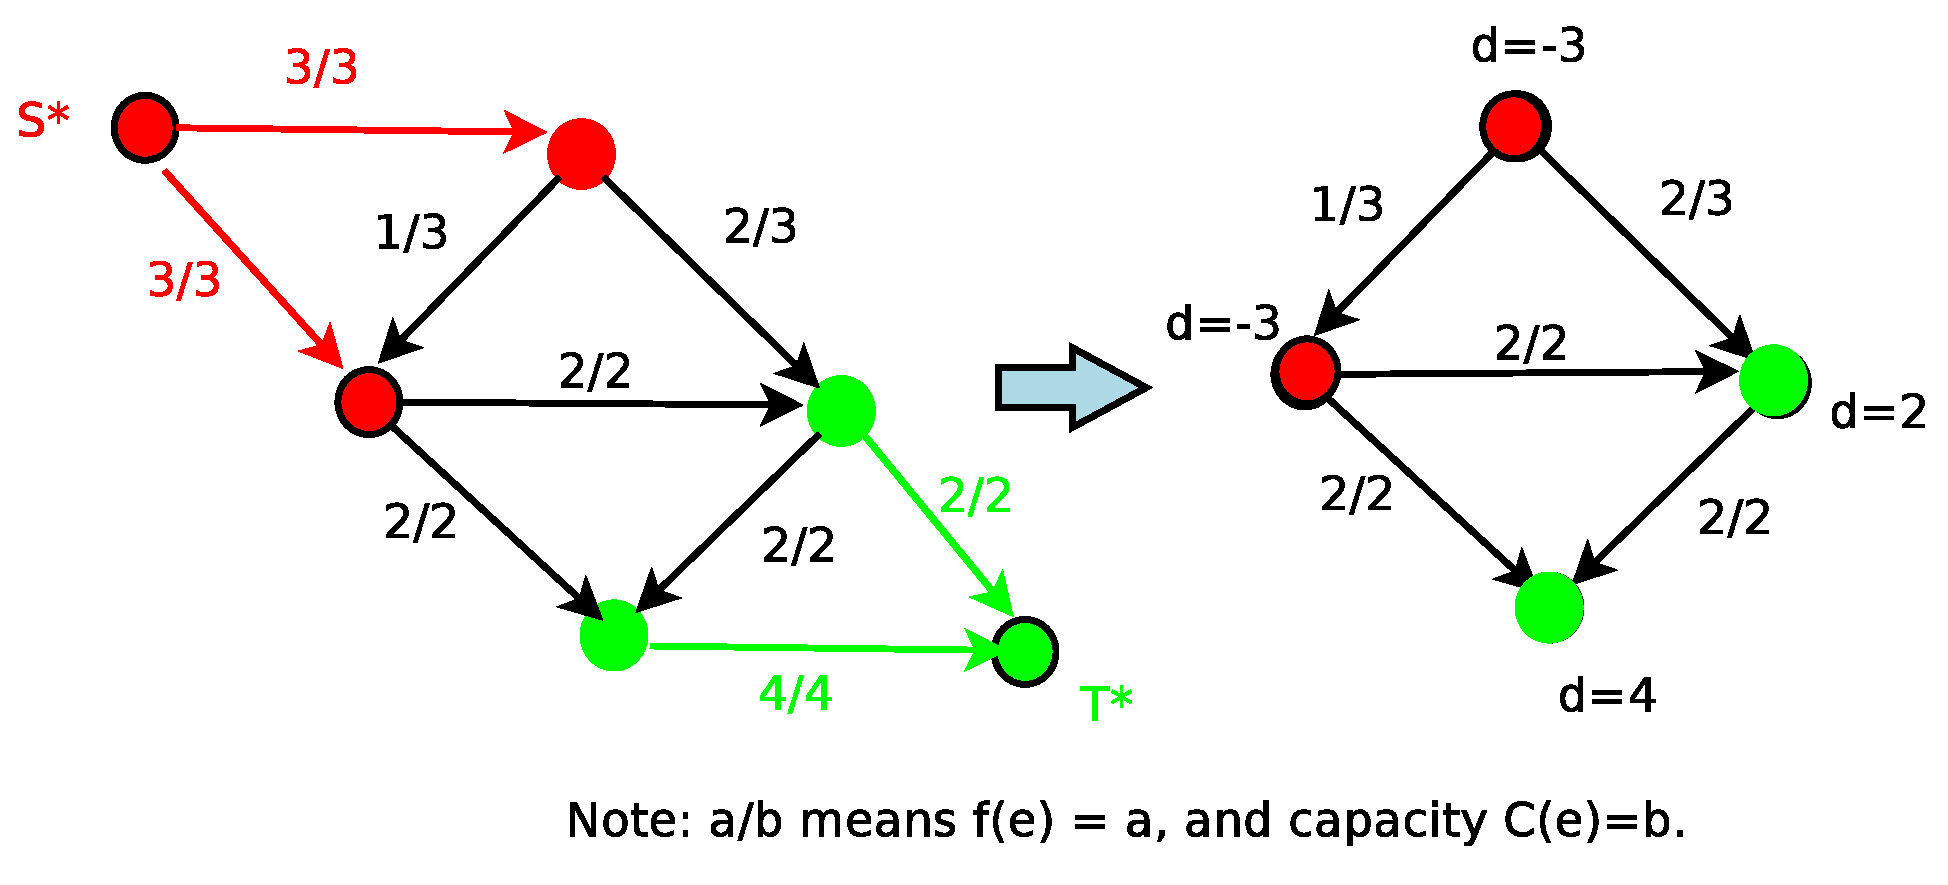
\includegraphics[width=3.5in] {L10-circulationtomaximumflowchecking.eps}
            \caption{检查$G'$上的最大流}
            \label{Figure: circulation_maximum_flow_checking}
        \end{figure}
        
       \subsubsection*{算法的正确性}
       \begin{theorem}
            流通问题存在一个可行解当且仅当图$G'$上的最大$s^*-t^*$流等于$D$.
        \end{theorem}
        \begin{proof}
        %\begin{itemize}
        \item $\Leftarrow$: \\
删除所有的$(s^*,s_i)$和$(t_j,t^*)$边. 显然所有$s_i$和$t_j$都满足容量限制和需求限制.
        \item $\Rightarrow$: 即如果我们能找到一个可行解, 那最大流肯定是$D$ \\
我们构造一个$s^*-t^*$流并证明这个流是最大流:
\begin{enumerate}
\item 定义一个流$f$如下: $f(s^*,s_i)=-d_i$且$f(t_j, t^*)=d_j$. 
\item 考虑一个割$(A,B)$, 其中$A=\{s^*\}$, $B=V-A$, 就是超级源点和其他顶点之间的割, 显然这个割的值是$C(A,B)=D$.
\item 我们有$C(A,B)=D$. 因为$f$达到了最大, 所以$f$是一个最大流.
\end{enumerate}
%\end{itemize}
        \end{proof}
        
        \subsection{每条边有流量下界的流通问题}
        \subsubsection*{问题的定义}
        \paragraph{}简单来说, 这里我们要求每条边上至少要运一定的货物, 完整的定义如下:
        \paragraph{输入: }一个图$G=<V, E>$, 每条边$e$都有一个容量{\bf 上界}$C(e)$和容量{\bf 下界}$L(e)$. 存在多个源点$s_i$和多个汇点$t_j$. 每个汇点$t_j$都有一个需求$d_j > 0$, 每个源点$s_i$可以提供$d_i$(可以表示为负的需求$d_i < 0$).
\paragraph{输出:}一个{\bf 可行流通(feasible circulation)} $f$, 它满足所有节点的需求限制, 也就是:
        %我这里翻译上不是很确切 to satisfy all demand requirements using the available supply, i.e.,
        \begin{enumerate}
        \item{容量限制:}  $L(e) \leq f(e) \leq C(e)$;
        \item{需求限制:}  $f^{in} (v) - f^{out} (v) = d_v$;
        \end{enumerate}
	    \paragraph{}为表述简单, 对所有既不是源点也不是汇点的节点$v$, 我们定义$d_v=0$. 由此, 我们有$\sum_i d_i = 0$. 同时我们令$D=\sum_{d_v >0 } d_v$为{\bf 总需求}.
	    \subsubsection*{一个例子}
	    \paragraph{}下面我们来举一个例子, 如\figurename\ref{Figure: lower_bound_circulation_example}所示, 跟之前问题的差别仅仅在于边$(s_1, s_2)$至少运$2$吨, 至多运$3$吨.
	    \begin{figure}[h]
	        \centering
            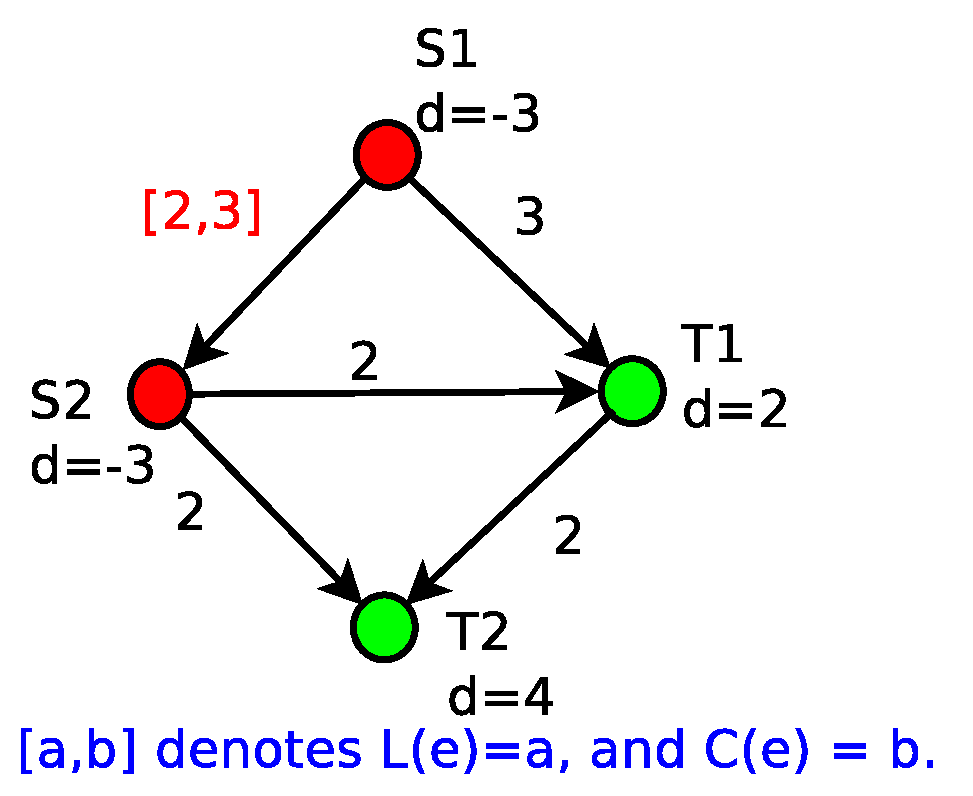
\includegraphics[width=2in] {L10-lowerboundcirculationexample.eps}
            \caption{带有流量下界的流通问题一个实例}
            \label{Figure: lower_bound_circulation_example}
        \end{figure}
\paragraph{} 流量的下界有一个很大的用途. 当我们设置了边$e$上的流量下界$L(e)>0$, 我们强制流使用边$e$. 例如,如\figurename\ref{Figure: lower_bound_circulation_example}所示, 流必须使用边edge $(s_{1}, s_{2})$. 大家在之后工作、研究中很有可能会遇到这样的问题: 这条路我必须得选. 这是一个很有意义的扩展.
        \subsubsection*{算法}
        \paragraph{}这个问题大家肯定可以做, 把之前写的线性规划中的$f(v,u) \geq 0$条件改成$f(v,u) \geq L(u,v)$就可以解决这个问题. 我们下面要讲的仅仅是让它更快一点.
        \paragraph{}解决这个问题的思想和之前几个问题是一样的, 有下界的我不会做, 我们看看能不能把这个下界给去了. 怎么去呢? 加一个初始的流. 过去我们从$0$流开始解网络流, 我们现在则从初始流开始. 具体如下:
        
        %\paragraph{}下面我们给出一个解决带流量下界的流通问题的有效算法.
        \begin{algorithmic}[1]
    \STATE 建立一个{\bf 初始流}$f_0$: 对所有边$e=(u,v)$, 令$f_0(e) = L(e)$; 
    \STATE 在图$G'$上解一个不带流量下界的流通问题. 特别的, 图$G'$是通过校正带有流量下界的边$e=(u,v)$建立的, 校正方法如下:
     \begin{enumerate}
     \item 顶点: $d'_u = d_u + L(e)$, $d'_v = d'_v - L(e)$,
     \item 边:  $L(e) = 0$, $C(e) = C(e) - L(e)$.
     \end{enumerate}
     令$f'$为图$G'$的可行流通.
    \STATE 返回 $f=f'+f_0$.
   \end{algorithmic}
   
        \subsubsection*{第一步: 建立初始流}
        \paragraph{}如\figurename\ref{Figure: lower_bound_circulation_step1_init_flow}所示, $(s_1, s_2)$边上至少要运$2$吨, 那我就让你把这$2$吨先运了, 这条边剩下的容量就是$1$. 而$s_2$本身就有$1$吨要往外运, 而预先运来了$2$吨, 就变成要运$3$吨了. 其他一切都没有变.
        \begin{figure}[h]
            \centering
            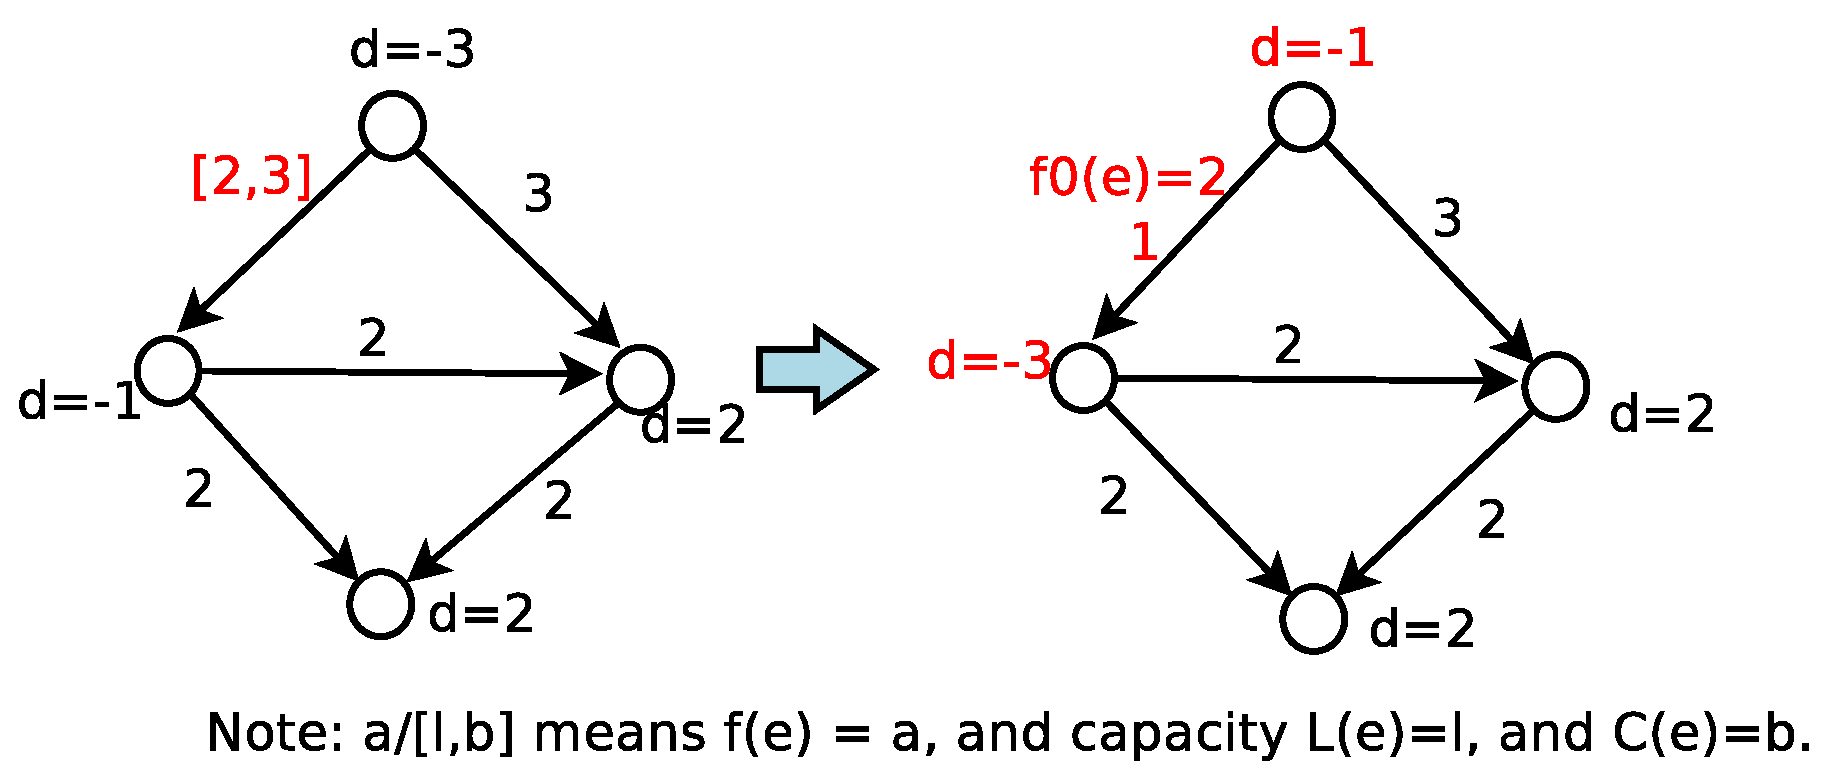
\includegraphics[width=3.8in] {L10-lowerboundcirculationstep1.eps}
            \caption{建立初始流, 最上面的顶点是$s_1$, 左面的是$s_2$}
            \label{Figure: lower_bound_circulation_step1_init_flow}
        \end{figure}
        \subsubsection*{第二步: 解一个新的流通问题}
        \paragraph{}经过初始流之后的问题就是我们之前讲过的流通问题, 再在这个网络$G'$上求得一个可行流通$f'$就行了, 如\figurename\ref{Figure: lower_bound_circulation_step2}.
        \begin{figure}[h]
            \centering
            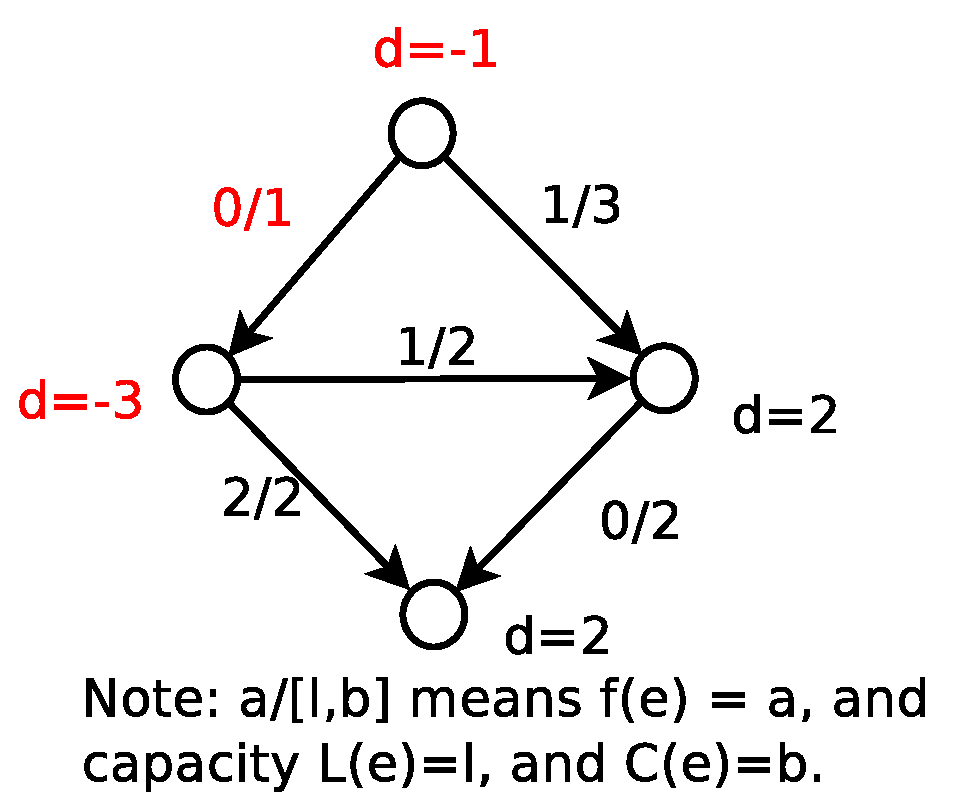
\includegraphics[width=1.8in] {L10-lowerboundcirculationstep2.eps}
            \caption{解$G'$上的流通问题}
            \label{Figure: lower_bound_circulation_step2}
        \end{figure}
        %\paragraph{}这样, 我们就在图$G'$上找到了一个可行流通$f'$.
        \subsubsection*{第三步: 将$f_0$和$f'$加起来}
        \paragraph{}最后, 如\figurename\ref{Figure: lower_bound_circulation_step3_adding}所示, 左侧第一个是初始流$f_0$, 第二个是上一步得到的可行流通$f'$. 把他们加起来, 我们就得到了原始问题的解$f = f_0 + f'$.
        \begin{figure}[h]
            \centering
            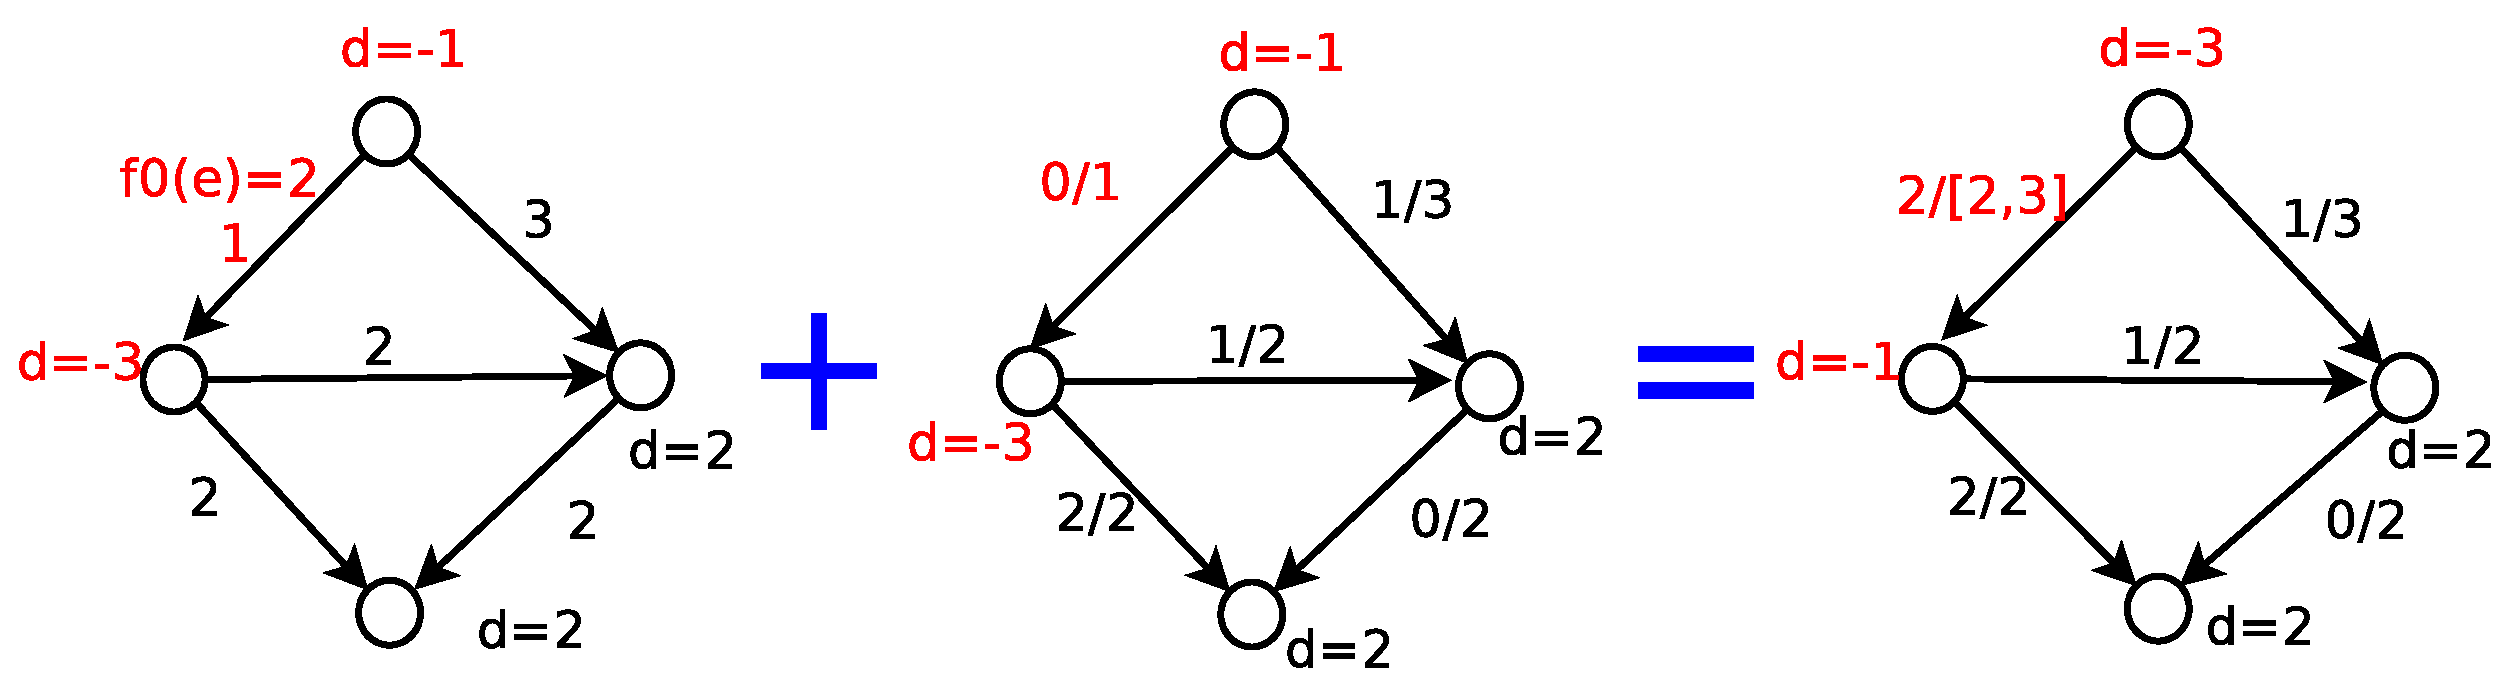
\includegraphics[width=4.5in] {L10-lowerboundcirculationstep3.eps}
            \caption{将$f_0$和$f'$加起来}
            \label{Figure: lower_bound_circulation_step3_adding}
        \end{figure}
        
        \subsubsection*{算法正确性}
        \paragraph{}接下来我们验证, 我们所得到的流满足问题所给的条件. 
        \begin{theorem}
        图$G$(带有流量下界)上有一个流通$f$当且仅当图$G'$(没有流量下界)上有一个流通$f'$.
        \end{theorem}
        \begin{proof}
%\begin{itemize}
\item 令$f'(e) = f(e)+L_e$.
\item 容易验证其满足容量限制和流通限制.
%\end{itemize}
        \end{proof}
        
        
    
    \subsection{最小费用流问题}
        \subsubsection*{问题的定义}
        \paragraph{输入:} 图$G=<V, E>$, 每条边$e$都有一个容量$C(e) > 0$和一个通过这条边上运送单位物品的{花费$w(e)$}. 存在两个特殊的节点: 源点$s$和汇点$t$. 从$s$到$t$运送流量为$v_0$.
        \paragraph{输出:}找一个流通$f$, 使得总流量等于$v_0$且花费最少.
        \subsubsection*{一个例子}
        \paragraph{}我们县来看一个例子, 如\figurename\ref{Figure: min_cost_flow_example}所示, 我们的目标是: 用最少的花费将$v_{0}=2$单位的货物从$s$运到$t$. 
        \begin{figure}[h]
            \centering
            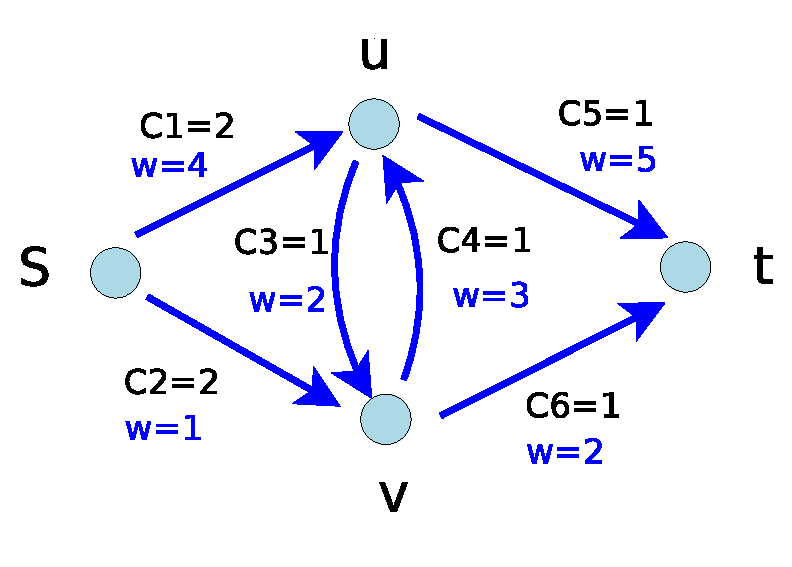
\includegraphics[width=1.8in]{L10-mincostflowexample.eps}
            \caption{最小费用流的一个实例}
            \label{Figure: min_cost_flow_example}
        \end{figure}
        \paragraph{}这个问题就不是那么容易了, 我们需要运一定的货, 使得花费的钱越少越好. 之前的一些例子我们一眼就能看出答案, 而这个例子, 没有办法直接看出答案. 为什么这么难呢, 主要是每条边上有个价钱$w_{e}$. 它把这个问题复杂化了. 同时我们也不能像之前几个问题那样简单的将图$G$转换为另一个$G'$. 怎么办呢? 我们就回到原始对偶的想法上去.
        \subsubsection*{原始对偶}
        \paragraph{}我们给每条边上设一个流量$y_{i}$代表边$i$运几吨, 由此写出\figurename\ref{Figure: min_cost_flow_example}中最小费用流的线性规划表达式如下:
%       这里的图和之前example一样

\[
\begin{array}{rrrrrrrllllll}
\textcolor{red}{\bf \min } &4y_1&+ y_2&+ 2y_3&+3y_4&+5y_5&+2y_6 &         &  \\
 s.t. & y_1 &+ y_2&    &    &      &      & \textcolor{red}{=}  2 &  \text{node } s \\
      &     &     &    &    &  -y_5 &-y_6 & \textcolor{red}{=}  -2 &  \text{node } t\\
      & -y_1 &     &+y_3&-y_4&+y_5 &      & \textcolor{red}{=}  0 &  \text{node } u\\
      &     & -y_2&-y_3&+y_4&   &+y_6 & \textcolor{red}{=}  0 &  \text{node } v\\
      &     &     &    &    &      &  y_i & \leq  C_i & \\
      &     &     &    &    &      &  y_i & \geq  0 & \\
\end{array} \nonumber
\]
        \paragraph{}我们已经把这个问题写成线性规划的形式了, 可以说这个问题就已经解决了. 下面的问题就只是有没有更快的解法? 我们使用下面的规则将这个线性规划重写为标准的对偶形式.
\begin{itemize}
 \item 目标函数: 将$\min$替换为$\max$.
 \item 限制: 将 ``$=$''替换为``$\leq$''. (注意到如果所有的不等式都满足的话, 它们都应当取等号. 例如, 不等式(2), (3)和(4)使得$y_{1} + y_{2} \geq 2$. 因此, 它将不等式(1)的$\leq$变成$=$. 其他不等式也是一样的.)
\end{itemize} 
        \paragraph{}可以得到如下的对偶形式:
\[
\begin{array}{rrrrrrrllllll}
\textcolor{red}{ \max } &-4y_1&-y_2&-2y_3&-3y_4&-5y_5&-2y_6 &         &   \\
 s.t. & y_1 &+y_2&    &    &      &      & \textcolor{red}{\leq}  2 &  \text{node } s  \\
      &     &     &    &    &-y_5 &-y_6 & \textcolor{red}{\leq}  -2 &  \text{node } t  \\
      &-y_1 &     &+y_3&-y_4&+y_5 &      & \textcolor{red}{\leq}  0 &  \text{node } u  \\
      &     &-y_2&-y_3&+y_4&   &+y_6 & \textcolor{red}{\leq} 0 &  \text{node } v  \\
      &     &     &    &    &      &  y_i & \leq  C_i &  &\\
      &     &     &    &    &      &  y_i & \geq  0 &  &\\
\end{array}
\]
        \paragraph{}回到我们的目标, 从$s$到$t$运$2$吨货物且花费最少. 那么首先, 第一个问题是不管价钱多少, 从$s$到$t$能不能运$2$吨货物. 第二问题, 在运$2$吨的条件下费用最小.
        \paragraph{}我们首先看第一个问题, 我们可以找到一个流量为$2$的流通. 这个很容易, 这就是一个流通问题, 我们之前已经解决了. 这样, 就相当于我们得到了原始对偶问题$D$的一个初始可行解.
        \paragraph{}接下来, 我们把这个初始可行解代进去, 看能不能接着进行改进, 这个就是我们原始对偶里最核心东西: DRP. 接下来, 我们就由对偶把这个问题的DRP写出来, 回想从原始对偶构造DRP的核心思想: 给一堆初始解$y_i$, 把他们全部代进对偶里去, 看是小于号还是等于号成立. 如果是等于, 在DRP中是对应的约束是小于等于:
        \begin{align*}
        y \text{: Dual: } & \sum ** = C_1 \\
        \Rightarrow \Delta y \text{: DRP: } & \sum ** \leq 0
        \end{align*}
如果是严格小于, DRP中这个约束就没了:
        \begin{align*}
        y \text{: Dual: } & \sum ** \leq C_2 \\
        \Rightarrow \Delta y \text{: DRP: } & \text{ empty}
        \end{align*}
这个的直观含义是, 我们要得到$y' = y + \theta \Delta y$, 而$y'$也要满足之前的约束, 即:
        \begin{align*}
            \sum ** \leq  C_1 \\
            \sum ** \leq  C_2
        \end{align*}
如果在对偶中是等于号(即$C_1$这个约束), 在DRP中是小于号, 加起来肯定小于等于$C_1$. 如果对偶中是小于号, 即已经小于$C_2$了, 这就意味着不等式左边和$C2$总有差值, 在DRP中就不用约束了, 因为我们总可以调节$\theta$使得对$y'$, $C_2$这个不等约束成立.
       \paragraph{}对这个问题而言, 具体规则如下: 
\begin{itemize}
 \item 将右边的项替换为$0$.
 \item 将$J$中没有的约束去除($J$包含了$D$中使$=$成立的那些约束).
 \item 对每条边增加约束$y_{i}  \geq -1$.
\end{itemize}
        %\paragraph{}或者说, 对这个对偶问题
\paragraph{}我们可以得到如下的DRP:
\[
\begin{array}{rrrrrrrlllllll}
 \max &-4y_1&-y_2&-2y_3&-3y_4&-5y_5&-2y_6 &         &  \\
 s.t. & y_1 &+y_2&    &    &      &      & \leq  0 &  \text{node } s \\
      &     &     &    &    & y_5 &+y_6 & \leq  0 &  \text{node } t\\
      & y_1 &     &-y_3&+y_4&-y_5 &      & \leq  0 &  \text{node } u\\
      &     &  y_2&+y_3&-y_4&  &-y_6 & \leq  0 &  \text{node } v\\
      &     &     &    &    &      &  y_i & \leq  0 & \text{for full arc}\\
      &     &     &    &    &      & -y_i & \leq  0 & \text{for empty arc}\\
      &     &     &    &    &      &  y_i & \leq  1 & \text{for any arc}\\
\end{array} \nonumber
\]
        \paragraph{}接下来, 先引入一个概念, 再回到DRP上.
        \begin{definition}[{\bf 环流(Cycle flow)}]
一个流$f$, 如果对任意节点(包括$s$和$t$), 流入等于流出, 那么它就被称为{\bf 环流(cycle flow) }.
        \end{definition}
        \paragraph{}如果我们已经得到了图$N$上的一个流, 那么我们把这个流带进去, 把它的DRP写出来, 接下来就是解这个DRP. 解这个DRP, 可以跑单纯性算法, 但对这个问题, 可以不用老老实实那么干, 这个问题是一个组合问题. 实际上, 解这个DRP与在一个新的图$N'(f)$中找一个圈等价. 图$N'(f)$构造方法如下:
\begin{enumerate}
 \item 对$N$中的每条边$e=(u,v)$, 在$N'(f)$中引入两条边$e=(u,v)$和$e'=(v,u)$;
 \item 将$N'(f)$中的边$e$和边$e'$的容量分别设置为$C(e)-f(e)$和$-f(e)$;
 \item 费用为$w(e')=-w(e)$;
\end{enumerate}
对每条边, 如\figurename\ref{Figure: min_cost_flow_cycle_flow}所示, $-w$对应的是退货边, 可以解释为最多可以把这$f$吨都退回来, 退一吨挽回之前的损失$w$元钱(过去的调度出错了), 也就是节省$w$元钱.
\begin{figure}[h]
    \centering
    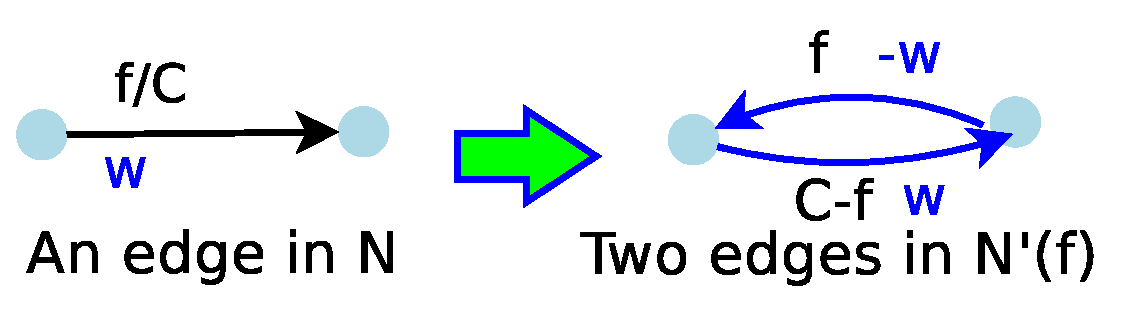
\includegraphics[width=2.5in] {L10-mincostflowNN.eps}
    \caption{构造$N'$}
    \label{Figure: min_cost_flow_cycle_flow}
\end{figure}
        \paragraph{}由上, 我们不用去解这个现行规划, 只要把原先的图变一下, 然后在这个图上面找有没有负圈. 这个正确性由如下的定理保证.
        \begin{theorem}
        $f$是图$N$上的最小费用流$\Leftrightarrow$图$N'(f)$中不包含带有负花费的圈.
        \end{theorem}
        \paragraph{}直觉上说, 如果网络$N'(f)$存在一个圈. 如果沿着这个圈推进一个单位流, 那么这个流就是一个环流(表示为$\overline{f}$). 那么$f+\overline{f}$仍然是原网络$N$的一个流.
        \begin{proof}
$f$是图$N$上的最小费用流 \\
$\Leftrightarrow$  $DRP$的最优解等于$0$.(也就是$\Delta y = 0$) \\
$\Leftrightarrow$  $N'(f)$中不包含带有负花费的环流(cycle flow).\\
$\Leftrightarrow$  $N'(f)$中不包含带有负花费的圈.
        \end{proof}
        
        \paragraph{}关于, DRP的最优解为$0$对应于$N'$中没有负圈, 大家可以结合后面的例子, 来看下面的说明: 这个DRP表达式就对应着几何的直观表达, 即这个图中有负圈. 首先第一点, DRP式子中, 对每个节点有$\leq 0$, 我们也已经说过, 这个等价于$=0$, 也就是说, 对每个节点而言, 流入等于流出. 这说明这个式子所表示的流是一个环流. 第二点, 它肯定是$N'$中的环流. $N'$体现在DRP不等中关于边的那三组不等式. 如果该边流量用完了, 那这条边就别用了, 即$y_i \leq 0$. 如果如果是空的边, 那还可以用. 第三点, 负圈, 体现在目标函数上.
        %我这里描述地不是很清楚

        \subsubsection*{算法}
        \paragraph{}M. Klein在1967年发明了一个最小费用流算法. 这个算法和我们之前看到的一样, 都是"改进"这个套路. 就是说, 一开始找一个初始解, 不断改进, 直到达到某个条件停止. 这个算法可以表示为:
        \begin{algorithm}[h]
        \caption{Klein algorithm}
        \label{algorithm: Klein algorithm}
\begin{algorithmic}[1]
    \STATE 使用最大流算法(比如Ford-Fulkerson算法)得到一个值为$v_0$的流$f$;
    \WHILE { $N'(f)$包含了一个负花费的圈$C$}
    \STATE 令$b$为圈$C$的bottleneck.
    \STATE 定义$\overline{f}$为$C$上的单位流.
    \STATE $f=f+b \overline{f}$;
    \ENDWHILE
    \RETURN $f$.
\end{algorithmic}
        \end{algorithm}
        \paragraph{}注意: 
        \begin{enumerate}
            \item 流上的花费随着迭代逐渐减少, 但同时流值保持不变.
            \item 带有负花费的圈可以通过Bellman-Ford算法来寻找.
        \end{enumerate}
        
        \paragraph{}下面我们来看一个例子:
        \subsubsection*{第一步}
        \paragraph{}建立一个初始流$f_0$: 流值为$2$, 流上的费用为: $17$. 如\figurename\ref{Figure: min_cost_flow_example_step1_init_flow}所示.
        
        \begin{figure}[h]
            \centering
            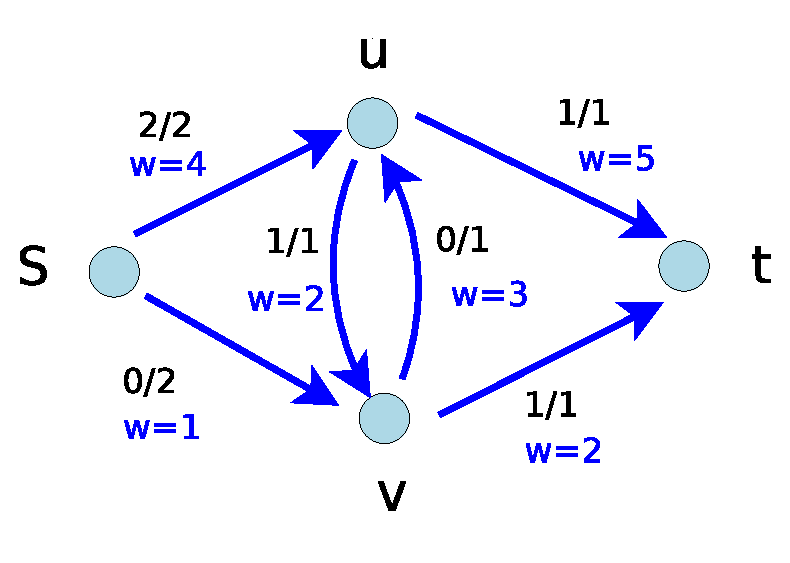
\includegraphics[width=1.5in] {L10-mincostflowexamplestep1.eps}
            \caption{建立初始流}
            \label{Figure: min_cost_flow_example_step1_init_flow}
        \end{figure}
        \paragraph{}接下来, 我们看这种方案能不能改进. 构造新图$N'(f)$, 如\figurename\ref{Figure: min_cost_flow_example_step1_Nprime}所示. 可以发现一个负费用圈:$s\rightarrow v\rightarrow u\rightarrow s$ (红色的部分). 费用为$-5$, 相当于挽回经济损失$5$元钱.
        \begin{figure}[h]
            \centering
            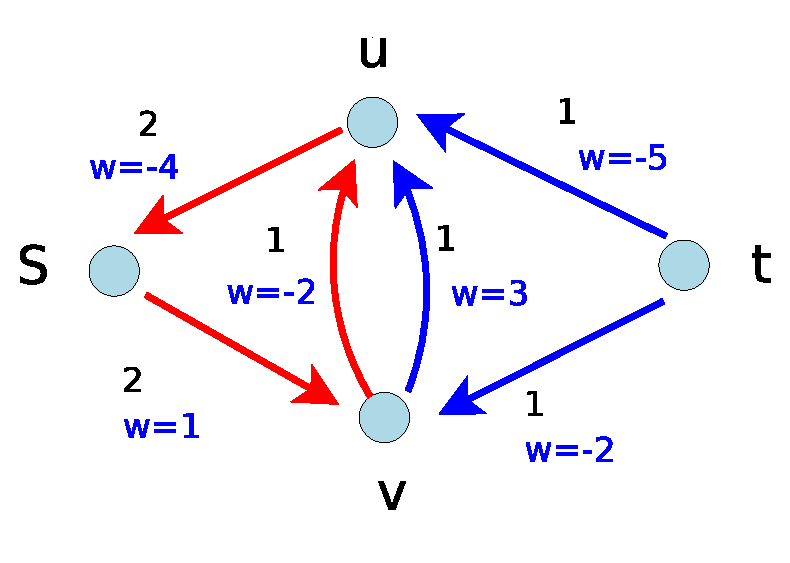
\includegraphics[width=1.5in] {L10-mincostflowexamplestep1N.eps}
            \caption{构造新图$N'(f)$}
            \label{Figure: min_cost_flow_example_step1_Nprime}
        \end{figure}
        
        \subsubsection*{第二步}
        \paragraph{}经过一轮迭代, 把上面得到的两个流加起来, 得到$f=f+\overline{f}$, 流值保持$2-0=2$, 费用为: $17-5=12$, 如\figurename\ref{Figure: min_cost_flow_example_step2}所示.
        \begin{figure}[h]
            \centering
            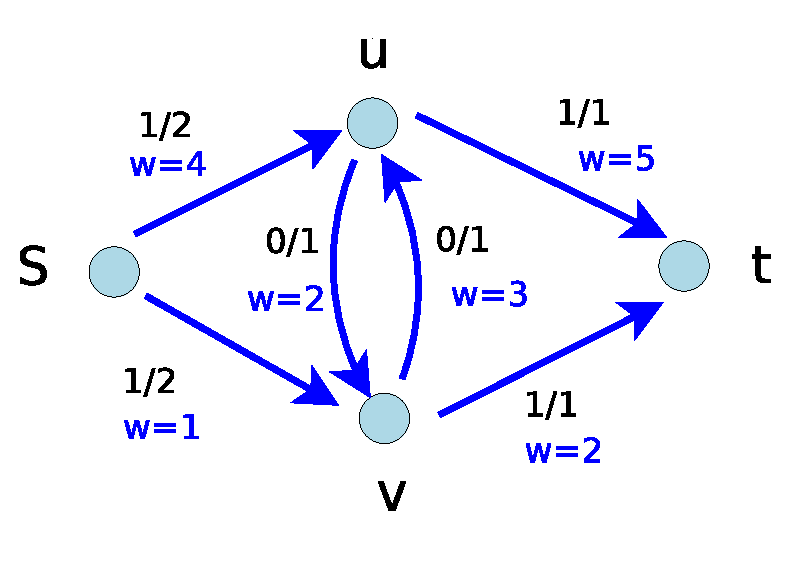
\includegraphics[width=1.5in] {L10-mincostflowexamplestep2.eps}
            \caption{迭代后的$N$}
            \label{Figure: min_cost_flow_example_step2}
        \end{figure}
        \paragraph{}再次构造$N'(f)$, 如\figurename\ref{Figure: min_cost_flow_example_step2_Nprime}所示. 可以发现图中没有负费用的圈了, 算法结束.
        \begin{figure}[h]
            \centering
            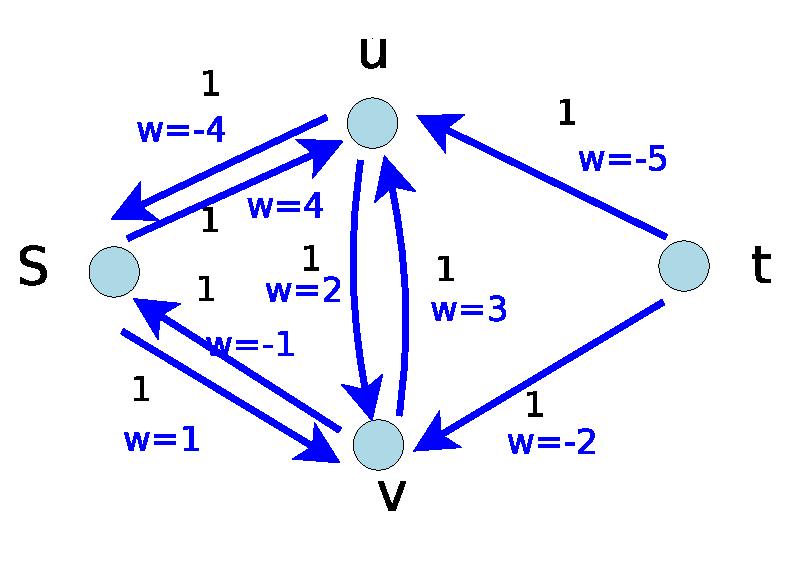
\includegraphics[width=1.5in] {L10-mincostflowexamplestep2N.eps}
            \caption{迭代后的$N'$}
            \label{Figure: min_cost_flow_example_step2_Nprime}
        \end{figure}
        \subsubsection*{扩展}
        \paragraph{}最小费用流有一个扩展, Hitchcock {\sc 运输(Transportation)}问题, 这个问题在1941年就已经提出来了, 问题定义如下:
        \paragraph{输入: } 存在$n$个源点$s_1, s_2, ..., s_n$和$n$个汇点$t_1, t_2, ..., t_n$. 每个源点$s_i$可以供应$a_i$, 每个汇$t_j$有一个需求$b_j$. $s_i$到$t_j$的费用是$c_{ij}$.
        \paragraph{输出: } 设计一种调度使得费用最少.

        \paragraph{}Frank L. Hitchcock在1941年提出了这个问题. 这个问题等价于最小费用流[Wagner, 1959]. 这个问题是一个最小费用流的特例, 这个图是一个二部图, 而最小费用流是一般图. 当每条边$c_{ij}=0/1$时, 这个问题就变成了分配问题.
\paragraph{}在1956年, L. R. Ford Jr.和D. R. Fulkerson提出了一种"标签"法来解决运输问题. 这个算法比单纯形效率高很多, 可以参见"Solving the Transportation Problem", L. R. Ford Jr. and D. R. Fulkerson.



\section{网络流的应用}
        \paragraph{} 为了将一个问题转化为网络流问题, 我们需要做以下几个工作:
        \begin{enumerate}
         \item 我们首先应该定义一个{\bf 网络(图)}. 有时原始问题有图, 我们只要改一下就行了, 而有时我们需要完全从头开始建立这个图.
         \item 接着我们需要定义{\bf 边上的权值}. 有时原始问题中权值在顶点上, 这时我们需要将顶点上的权值移到边上.
         \item 定义{\bf 源点$s$}和{\bf 汇点$t$}. 有时我们需要定义超级源点$s^*$和超级汇点$t^*$.
         \item 最后我们需要证明{\bf 最大流} (寻找路径、匹配)或{\bf 最小割} (划分节点)正好是我们想要的, 这个是最重要的.
        \end{enumerate}
        \paragraph{}注意: 大多数问题都用到了这么一个性质: 存在一个整数值的最大流当且仅当存在一个最大流.
        \paragraph{}那什么样的问题天然能想到它是一个最大流呢? 一方面, 考虑最大流. 所谓流, 就是一堆$s$到$t$的路径(或者说通路), 所以如果让我们在图中找路径, 我们可以想到最大流. 如果找到一条边, 这是一个匹配的话, 那这也是一个天然的最大流问题. 另一方面, 考虑最小割. 所谓割就是把顶点分成两堆, 所以如果原始问题让我们把顶点分成几个部分的话, 那我们就可以想到割.
        
    \subsection{集合划分}
        \paragraph{} 第一个问题, 加入问题让我们把一个集合分成两半, 这个时候我们就可以想到网络流(最小割). 我们来看几个例子:
        \subsubsection{图片分割问题}
%            \subsubsection*{问题的定义}
\begin{figure}[h]
                 \centering
                 
\includegraphics[width=1.0in]{L10-image-Einstein.png}
                 \caption{一幅像素图}
                 \label{Figure: image_segmentation_einstein_pixel}
             \end{figure}
\paragraph{}我们首先来看一张图片, 如\figurename\ref{Figure: image_segmentation_einstein_pixel}所示, 相信大家都看得出来这是谁, 为什么能看出来呢? 因为虽然我们没有意识到, 我们的大脑对每一像素都分辨了一次这个是前景还是背景. 那些很亮的点基本都是前景, 很暗的点基本都是背景. 而有的点我们可能一下子无法分辨, 但是他们周围存在一些跟他们很像的点, 这是我们可以说, 这个点和田周围的这个点同属于背景或同属于前景. 这就是图片分割({\sc ImageSegmentation})问题, 定义如下:
            \paragraph{输入:} 给定一个像素图格式的图像(比如\figurename\ref{Figure: image_segmentation_einstein_pixel}). 像素$i, i\in P$有一定概率$f_i$是前景, 有有一定概率$b_i$是北京. 另外,两个相邻的像素$i$和$j$相似的概率是$l_{ij}$;
            \paragraph{目标:}将前景从背景中辨识出来. 形式化的, 我们希望得到一个划分$P=F\cup B$($F$表示前景, $B$表示背景), 使得$Q(F, B) = \sum_{i\in F} f_i + \sum_{j\in B} b_i + \sum_{i \in F}\sum_{j \in N(i)\cap F} l_{ij} + \sum_{i \in B}\sum_{j \in N(i)\cap B} l_{ij}$最大.
            \paragraph{}目标中的$Q(F, B)$是什么意思呢, 是以下三者之和: 你认为是前景的那些像素是前景的概率, 你认为是背景的那些像素是背景的概率, 以及所有前景中邻居也是前景的概率和所有背景中邻居也是背景的概率. 为什么要最大化这个呢? 如果大家学过机器学习有关的课程, 大家就会明白他是再做一个极大似然. 我们假设$x_i=0$表示$i$像素是背景, 而$x_i=1$表示是前景. $X$表示所有像素的$x_i$组成的向量. 我们其实是在$max$  $P(X|f,l)$. 我们把这个概率写成能量的指数(或者说能量是概率的负对数), 再把能量展开, 有:
            \begin{align*}
           \text{max  } & P(X|f, l) \\
            =& e^{-E(x)}  \\
            =& \exp{\{-(\sum_i {P_i(x_i)} + \sum_i \sum_j h_{ij}(x_i, x_j))\}}
            \end{align*}
            很多东西都能写成这个样子, $E(x)$展开玻尔兹曼分布, 为什么呢? 它是从最大熵来的. 这个玻尔兹曼分布, 我们一般就写单体项和两体项, 三体项样本数量已经不够了. 而上面那个最大似然就相当于:
            \begin{align*}
            \text{min  } \sum_i {P_i(x_i)} + \sum_i \sum_j h_{ij}(x_i, x_j)
            \end{align*}
            这里补充一点:
            \begin{align*}
            \begin{cases}
            P(x) = e^{-E(x)} \\
            E(x) = -\log{P(x)}
            \end{cases}
            \end{align*}
            大家熟悉的是概率取负对数是熵, 在这里概率取负对数是能量. 其实, 熵就是不能做功的能量.
            \paragraph{}回到目标中的目标函数$Q(F, B)$, 大家知道这个是由极大似然来的, 不是瞎设的. 现在我们就不管为什么写成这样的, 考虑怎么解这个问题. 这个问题大家可以写成优化问题, 但是, 很不幸的, 无法直接写成线性规划的形式, 直接写是一个二次优化的问题(两个求和那里得用$x_i x_j$). 
             
            %\subsubsection{一个例子}
            \paragraph{}接下来, 我们先看一个有$9$个像素的例子, 如\figurename\ref{Figure: image_segmentation_example}所示. 
            \begin{figure}[h]
                \centering
                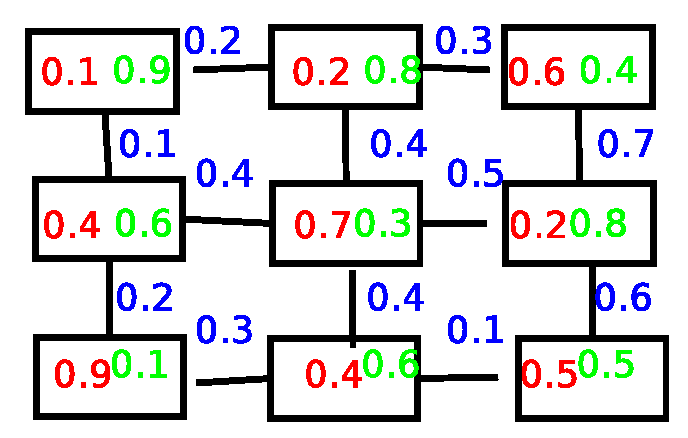
\includegraphics[width=2in]{L10-image-example1.eps}
                \caption{一个图片分割的实例}
                \label{Figure: image_segmentation_example}
            \end{figure}
\paragraph{}每个格子代表一个像素, 其中:
 \begin{itemize}
 \item
  红色(每个格子的左侧): 像素$i$是前景的概率$f_i$;
  \item
   绿色(每个格子的右侧): 像素$i$是背景的概率$b_i$;
   \item
    蓝色(格子之间): 像素$i$和$j$在同一类的概率$l_{ij}$;
     \end{itemize}
        \paragraph{}这里需要把节点分成两堆, 这个我们就可以想到最大流最小割. 接下来我们按之前的四步把这个问题转化成一个网络流问题.
\begin{enumerate}
 \item 网络: 如\figurename\ref{Figure: image_segmentaion_exmaple_networkflow}所示,增加两个节点: 源点$s$和汇点$t$, $s$指向所有的像素, 所有的像素都指向$t$;
 \item 容量: 将像素(顶点)上的权值移到边上, 即$C(s,v)= f_v$, $C(v,t)= b_v$; $C(u,v)=l_{uv}$;
 \item 割: 对应一个划分.  割容量$C(F, B) = M - Q(F, B)$, 其中$M=\sum_i (b_i + f_i) + \sum_i\sum_j l_{ij}$是一个常数.
 \item 最小割: 原问题的最优解
\end{enumerate}
                \begin{figure}[h]
                    \centering
                    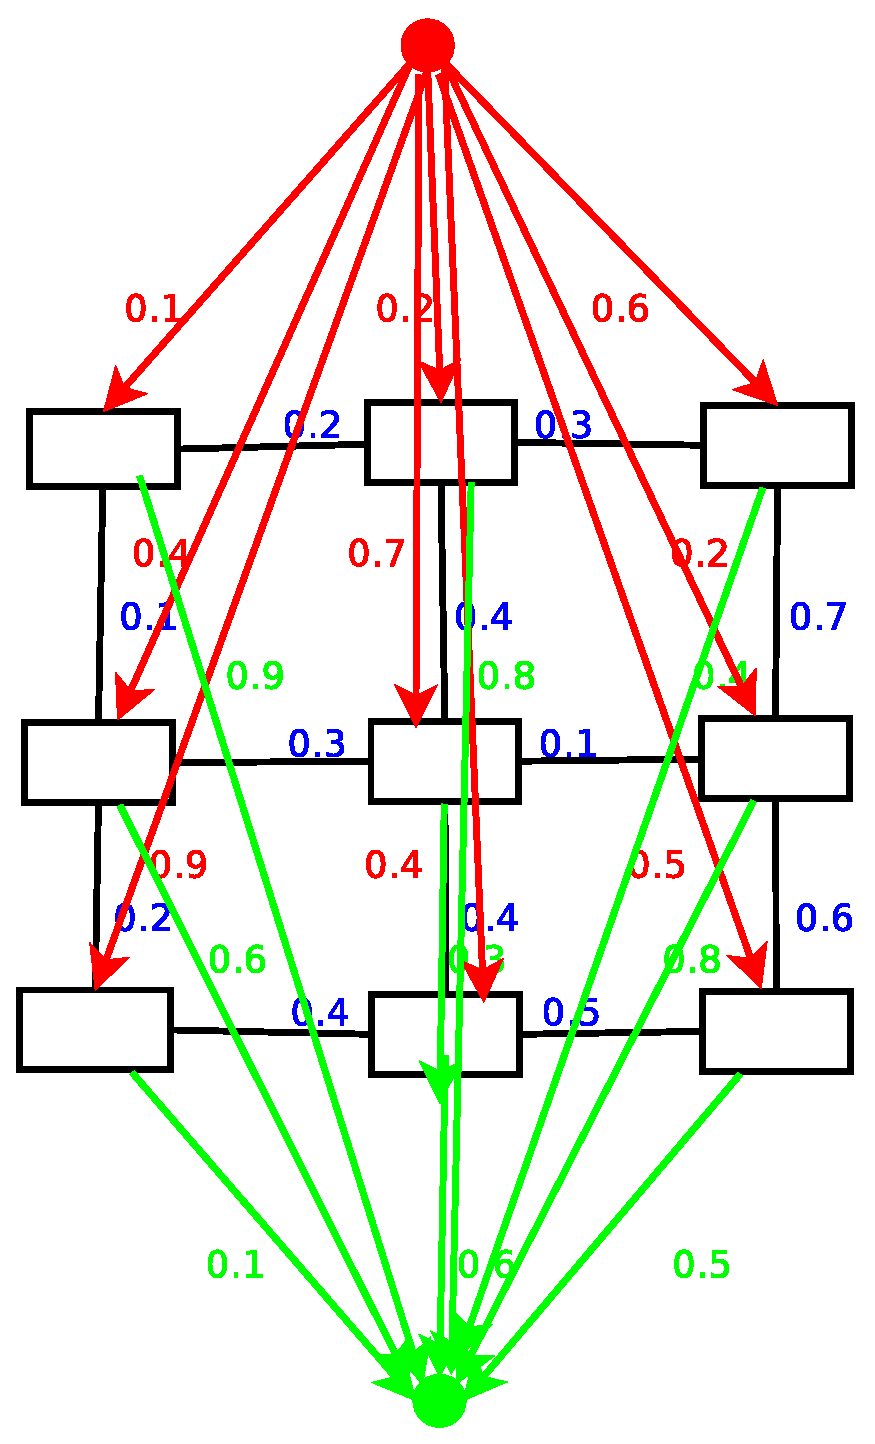
\includegraphics[width=1.2in]{L10-image-example1-network.eps}
                    \caption{将图片分割问题转化成网络流}
                    \label{Figure: image_segmentaion_exmaple_networkflow}
                \end{figure}
        \paragraph{}其中, 对割, 我们举一个例子, 比如第二三行之间的一个割, 我们认为上方的都是前景, 下方的都是背景的. 考察这个割所割的各种颜色的边的数目, 结合目标函数$Q(F,B)$中计数的边的数目, 将对应颜色的边相加, 正好是所有边的数目, 是个常数, 如\tablename\ref{Table: image_section_cut_and_objective}所示.
        \begin{table}[h]
        \centering
        \caption{割与目标函数对应的边的比较}
        \label{Table: image_section_cut_and_objective}
        \begin{tabular}{l|ccc}
        \hline
                 & 红边 & 蓝边 & 绿边 \\
        \hline
        $C(F,B)$ & $3$  & $3$  & $6$  \\
        $Q(F,B)$ & $6$  & $9$  & $3$  \\
        \hline
        $M= C+Q$      & $9$  & $12$ & $9$ \\
        \hline
        \end{tabular}
        \end{table}
        \paragraph{}而我们想要最大化$Q(F,B)$, 就等价于最小化$C(F,B)$, 也就是再求最小割. 这样, 这个问题就可以用最大流来解了, 这是一个比较快的方法. 但是, 我个人并不是特别推崇这个方法, 这个东西有点巧妙, 想出来就想出来了, 想不出来还是想不出来, 启发性不是很大. 我还是希望大家可以把这个问题写成线性规划或是二次规划. 事实上对之前提到的二次规划, 稍加技巧就可以把它写成现行规划.

        \subsubsection{工程选择问题}
            \paragraph{}我们首先给出工程选择{\sc Project Selection}问题的定义
            \paragraph{输入:}给定一个有向无环图(DAG).一个节点$i$代表一个工程, 完成这个工程将获得一定收益(表示为$p_i > 0$), 或者一定损失(表示为$p_i < 0$). 一条有向边$u \rightarrow v$表示先序条件(prerequisites), 比如$v$应当在$u$之前完成(即要想干$u$必须先干$v$). 
\paragraph{目标:}选择一个工程的子集$A$使得:
 \begin{enumerate}
    \item 可行: 如果一个工程被选中了, 那么他所有的先决工程也要被选中;
    \item 最优: 最大化利润$\sum_{ v \in A} p_v$;
\end{enumerate}

            \paragraph{}我们来看一个例子, 如\figurename\ref{Figure: project_selection_example_network}左面所示, 这个大家可以看做找工作时一年挣$10$万, 但是得先交$3$年学费, 一年$1$万. 问题就是在满足先序关系的条件下选择一些工程, 使得赚得钱越多越好.
            \paragraph{}先看一个巧妙的办法, 这个问题有是让我们在一个集合中选一个子集, 这就是割. 我们把它转换成一个网络流的问题, 构造流网络, 如\figurename\ref{Figure: project_selection_example_network}所示, 具体方法如下:
            \begin{enumerate}
 \item 网络: 原网络中没有源点和汇点, 引入连个节点: 源$s$和汇$t$, $s$指向所有赚钱($p_i > 0$)的节点, 所有交学费($p_i < 0$)的节点指向$t$;
 \item 容量: 将顶点上的权值移到边上, 并设$C(u,v)=\infty , \forall <u,v>\in E$.
 \item 割: 顶点集的划分.
            \end{enumerate}
            \begin{figure}[h]
                \centering
                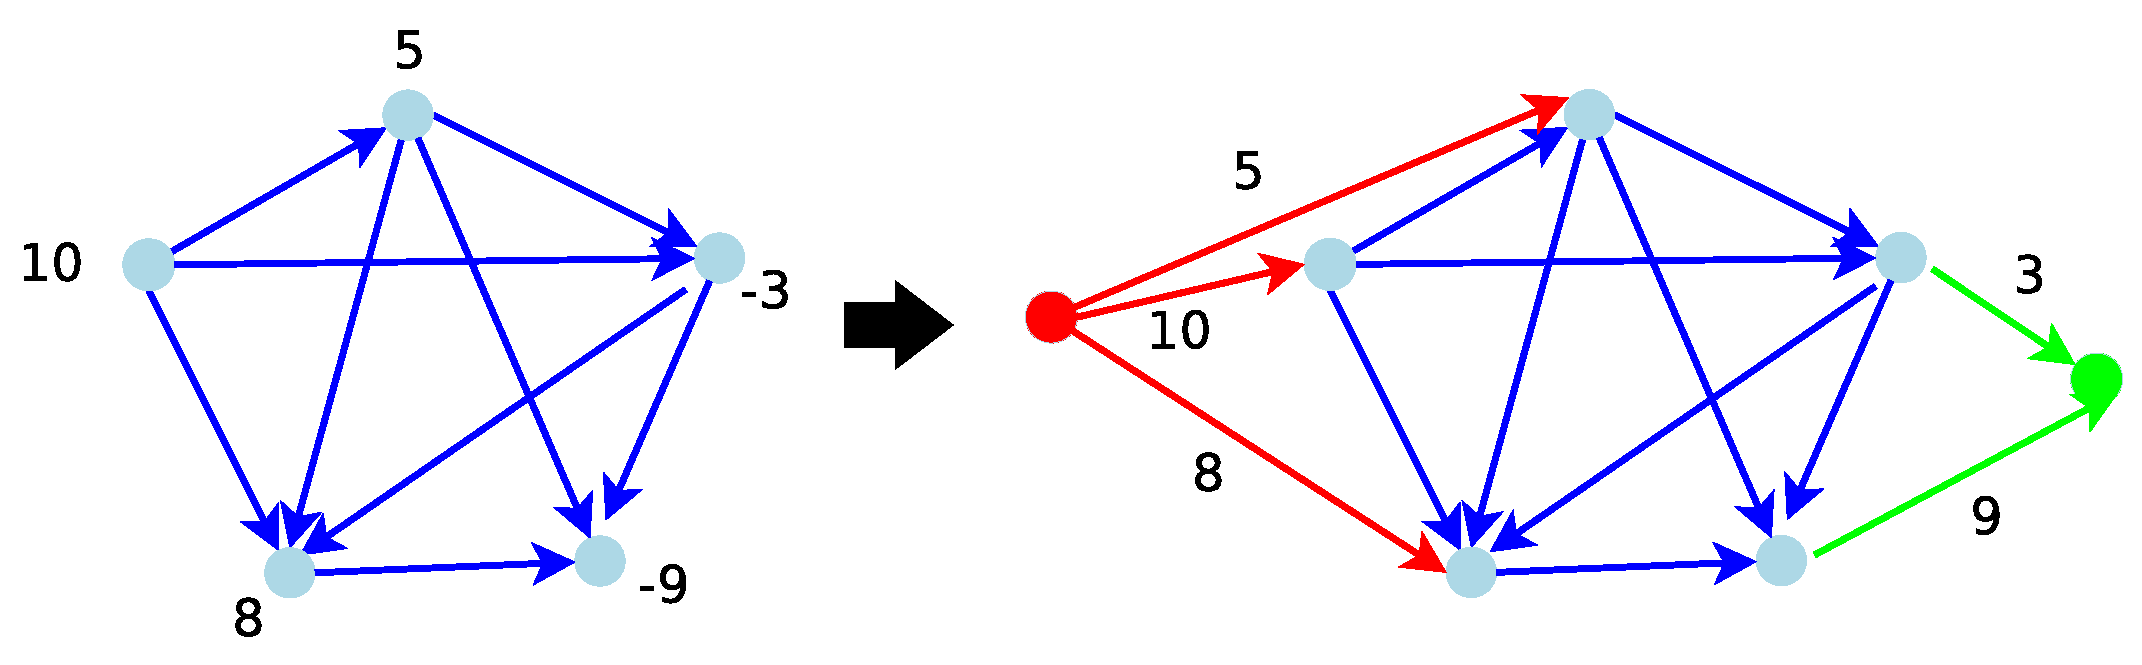
\includegraphics[width=3.3in]{L10-projectselectionexample-network.eps}
                \caption{构造流网络}
                \label{Figure: project_selection_example_network}
            \end{figure}

            \paragraph{}最终我们想说明最小割等价于最大利润. \figurename\ref{Figure: project_selection_example_network_cut}显示了实例上的一个割.
            \begin{figure}[h]
                \centering
                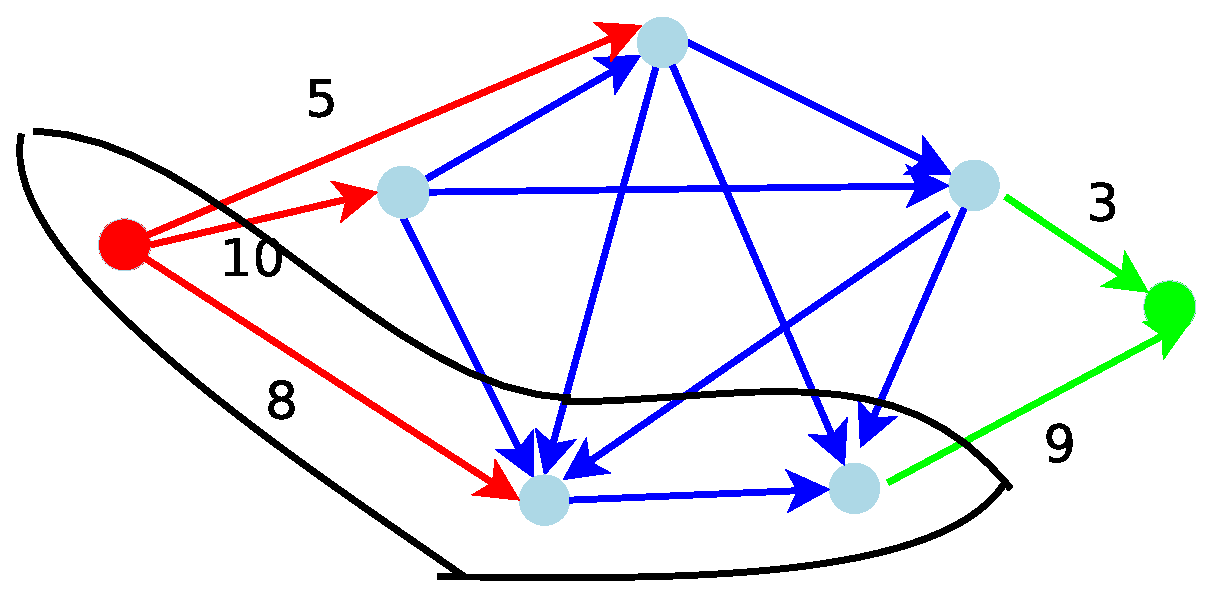
\includegraphics[width=2.5in]{L10-projectselectionexample-network-cut.eps}
                \caption{流网络上的一个割, 表示我们选择下面连个工程}
                \label{Figure: project_selection_example_network_cut}
            \end{figure}
            \paragraph{}这个例子所示的割容量为$C(A,B) = 5 + 10 + 9$, 而这个割表示选择下面两个(即全出来的两个)工程, 这个割对应的收益是$ \sum_{i \in A} p_i = 8 - 9 = -1 $. 这两个数加起来是$C = (5 + 10 + 9) + (8 - 9) = 5 + 10 + 8$, 是一个常数, 这个是所有能赚钱的项目之和, 就是\figurename\ref{Figure: project_selection_example_network_cut}左边三条红线上权值的和. 这个问题跟之前一个很像, 加起来等于常数, 要最大化收益, 只要最小化割就可以了. 对应于一般情况, 我们可以表述如下:
            \begin{enumerate}
 \item 割容量: $C(A,B) = C - \sum_{i \in A} p_i$, 其中 $C=\sum_{v\in V} p_v $ $(p_v > 0)$是一个常数.
  \item 最小割: 由于个容量和利润的和是一个常数, 所以最小割对应于最大利润.
            \end{enumerate}
            \paragraph{}最后, 还有一点微妙的东西, 我们为什么要把内部的边容量设成是$\inf$呢? 因为我们要保证这个解是可行的. 我们考察一个如\figurename\ref{Figure: projecgt_selection_example_network_cut_infeasible}所示的割, 在这个割中, 工程$u$被选中了, 但他的前导工程$v$没有被选上, 也就是说, 这个割是不可行的. 而在正中情况下, 那么边$<u,v>$就是一个割边, 这将使得我们得到的割容量为无穷. 这也就意味着, 求最小割我们是永远求不出这种情况的. 这也就强迫我们选取一个工程的前导工程, 这也是一个比较巧妙的地方.
            \begin{figure}[h]
                \centering
                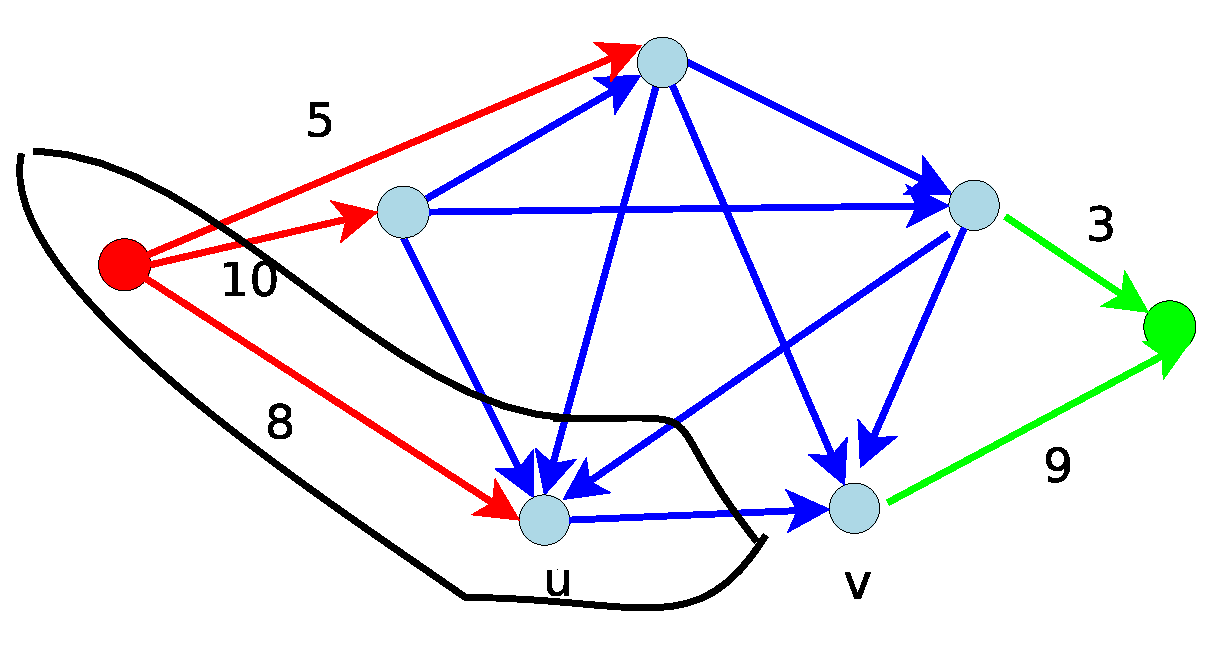
\includegraphics[width=2.5in]{L10-projectselectionexample-network-cut-infeasible.eps}
                \caption{一种不可行的割}
                \label{Figure: projecgt_selection_example_network_cut_infeasible}
            \end{figure}
            \paragraph{}那么, 这个设计这么巧妙, 想不出来怎么办? 我们还是回到线性规划上来. 我们对每一个工程设一个$x_i$表示该工程选还是不选. 而对先序关系, 比如完成$x_1$需要先完成$x_2$,我们有逻辑表达式: If $x_1$ then $x_2$, 这个等价于$x_2 \geq x_1$, 其他的边也同理. 这样对例子中的问题, 我们有以下的线性规划表达式:
            \begin{equation*}
\begin{array}{cl@{}ll}
\text{Max}  & 10x_1 + 5x_2 - 3x_3 - 9 x_4 + 8 x_5 &\\
\text{s.t.} & x_i = 0/1,\; i = 1,\dots,5  &\\
            & x_2 \geq x_1 &  \\
            & x_3 \geq x_1 &  \\
            & \dots
\end{array}
            \end{equation*}
            \paragraph{}这样, 如果大家觉得之前的精巧的做法想不到, 我们还可以用如上的线性规划来求解.

            
            
    \subsection{寻找路径}
        \paragraph{}之前我们已经讲了: 割就是把一个集合分成两堆. 那么流呢? 流就是从$s$到$t$经过一堆路径. 所以如果让我们从$s$到$t$找一堆路径的话, 我们可以想到最大流最小割.
        \subsubsection{不相交路径问题}
        \paragraph{我们来看一个问题: 不相交路径. 定义如下:}
        \paragraph{输入:}给定一张图$G=<V,E>$, 两个顶点$s$和$t$, 一个整数$k$.
        \paragraph{目标:}指定$k$个互不相交的$s-t$路径;
        \paragraph{}\figurename\ref{Figure: disjoint_path_example}展示了不相交路径问题的一个实例, 在这个例子中, 最多可以找到$4$条从$s$到$t$的不相交路径. 这个问题与图连接问题也有关. 
        \begin{figure}[h]
            \centering
            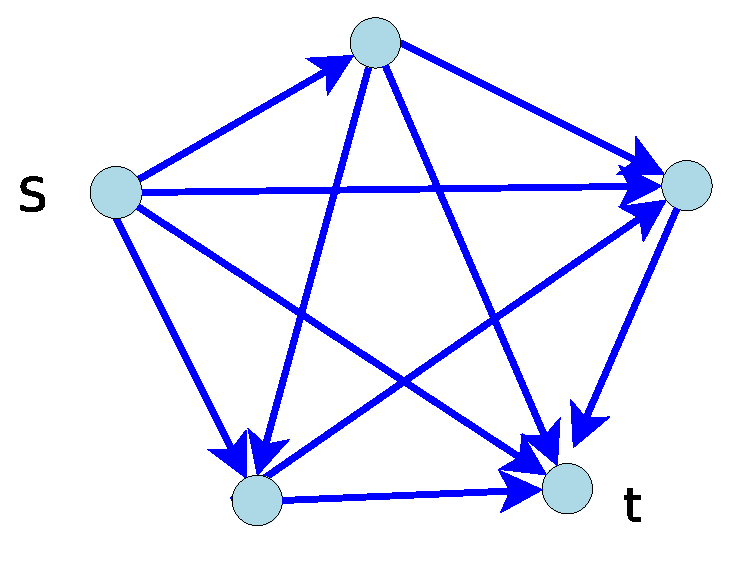
\includegraphics[width=1.5in]{L10-disjointpathsexample.eps}
            \caption{不相交路径问题的一个实例}
            \label{Figure: disjoint_path_example}
        \end{figure}
        
        \paragraph{}为了用网络流解决这个问题, 我们构造网络如下:
        \begin{enumerate}
         \item 边: 跟原图一样(原图已经天然给定了$s$和$t$);
         \item 容量: $C(u,v)=1$;
         \item 流: 如下所述%源PPT是(See extra slides).
        \end{enumerate}
        \paragraph{}注意, 每条边的流量都是$1$, 这就限制了每条边只能走一遍, 这就限制了各个路径不会有重叠(即相交).
        \begin{figure}[h]
            \centering
            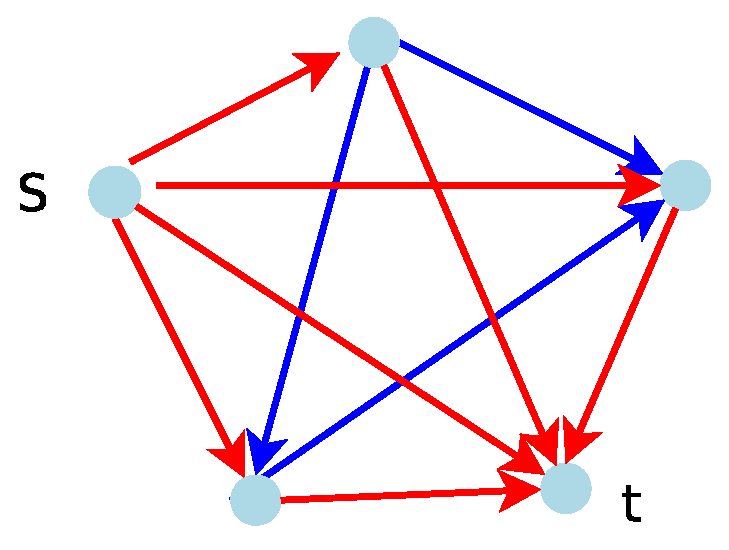
\includegraphics[width=1.3in]{L10-disjointpathsexample-number.eps}
            \caption{例子中得到的$4$个不相交的路径}
            \label{Figure: disjoint_path_example_number}
    \end{figure}
\begin{theorem}
图$G$中存在$k$割不相交的路径$\Leftrightarrow$ 最大的$s-t$流第值至少是$k$.
\end{theorem}
\begin{proof}
 \begin{enumerate}
  \item 注意: 最大$s-t$流值是$k$意味着这是一个值为$k$的整数流(不会出现$0.5$这样的非整数解).
  \item 选择$f(e) = 1$的变就行.
 \end{enumerate}
\end{proof}
            \paragraph{}关于时间复杂度, Ford-Fulkerson算法的复杂度为$O(mC)$, 而这里的$C$最多是$n$, 所以这个算法的时间复杂度为$O( mn)$.
            \paragraph{}上面这个问题很简单, 我们介绍一点扩展, Menger在1927年做了一个定理, 这个定理就是说不相交路径的最大数目等于我们小时候做的一个游戏: 把这些边想象成火柴棍, 拿掉几根以后$s$和$t$就不通了. 最小的火柴棍的数目等于最大的不相交路径数目, 形式化的表述如下:
            \begin{figure}[h]
                \centering
                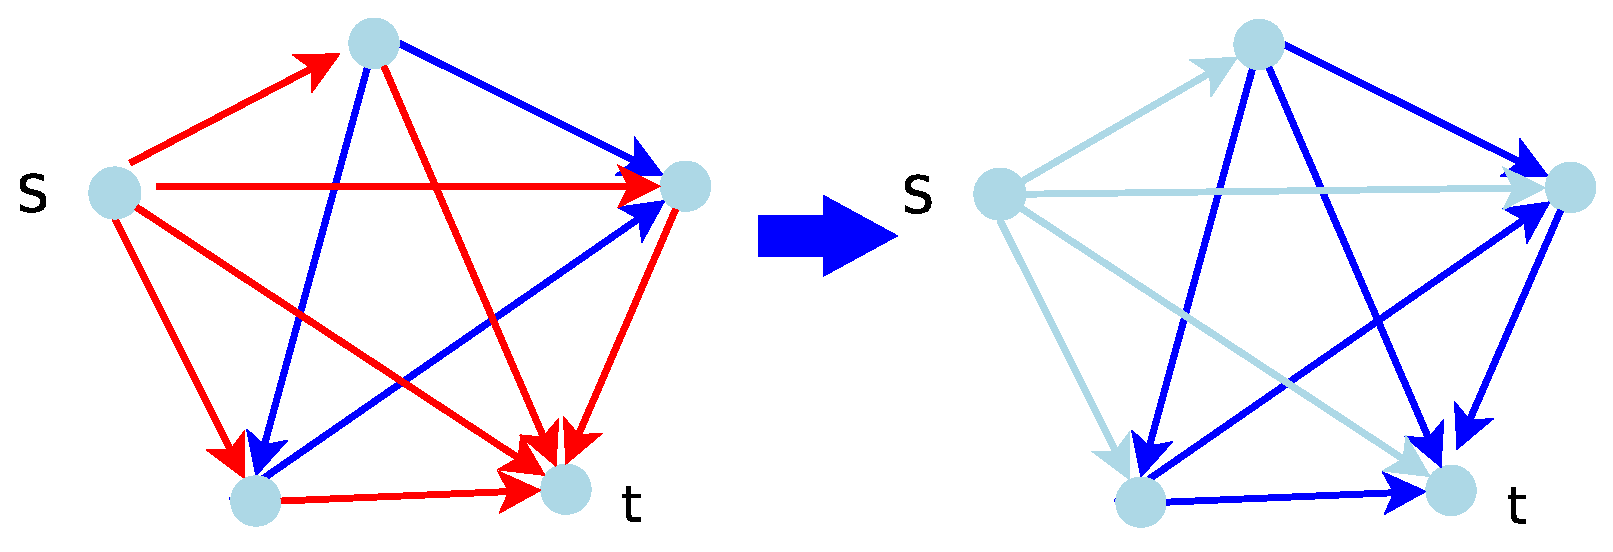
\includegraphics[width=2.7in]{L10-disjointpathsexample-Menger.eps}
                \caption{•}
            \end{figure}
\begin{theorem}[(Menger theorem)]
最大不相交路径的数目等于将$s$和$t$分隔开所需要删除的最小边数.
\end{theorem}
\begin{proof}
 \begin{enumerate}
  \item 最大不相交路径的数目等于最大流;
  \item 存在一个割$(A,B)$, 使得$C(A,B)$等于不相交路径的数目;
  %Then there is a cut $(A,B)$ such that $C(A,B)$ is the number of disjoint paths;
  \item 这个割的割边就是我们想要的那些边.
 \end{enumerate}
\end{proof}
        \subsubsection{调查问卷设计}
            \paragraph{}寻找路径路径问题还有一个应用, 调查问卷的设计, 定义如下:
            \paragraph{输入:} 顾客的集合$A$, 产品的集合$P$. 令$B(i) \subseteq P$表示顾客$i$购买的产品. 一个整数$k$.
            \paragraph{目标:} 设计一个有$k$个问题的调查问卷, 使得对顾客$i$, 问题的数量至少是$c_i$, 至多是$c'_i$. 另一方面, 对每种产品, 问题的数目至少是$p_i$, 至多是$p_i'$.
        \begin{figure}[h]
            \centering
            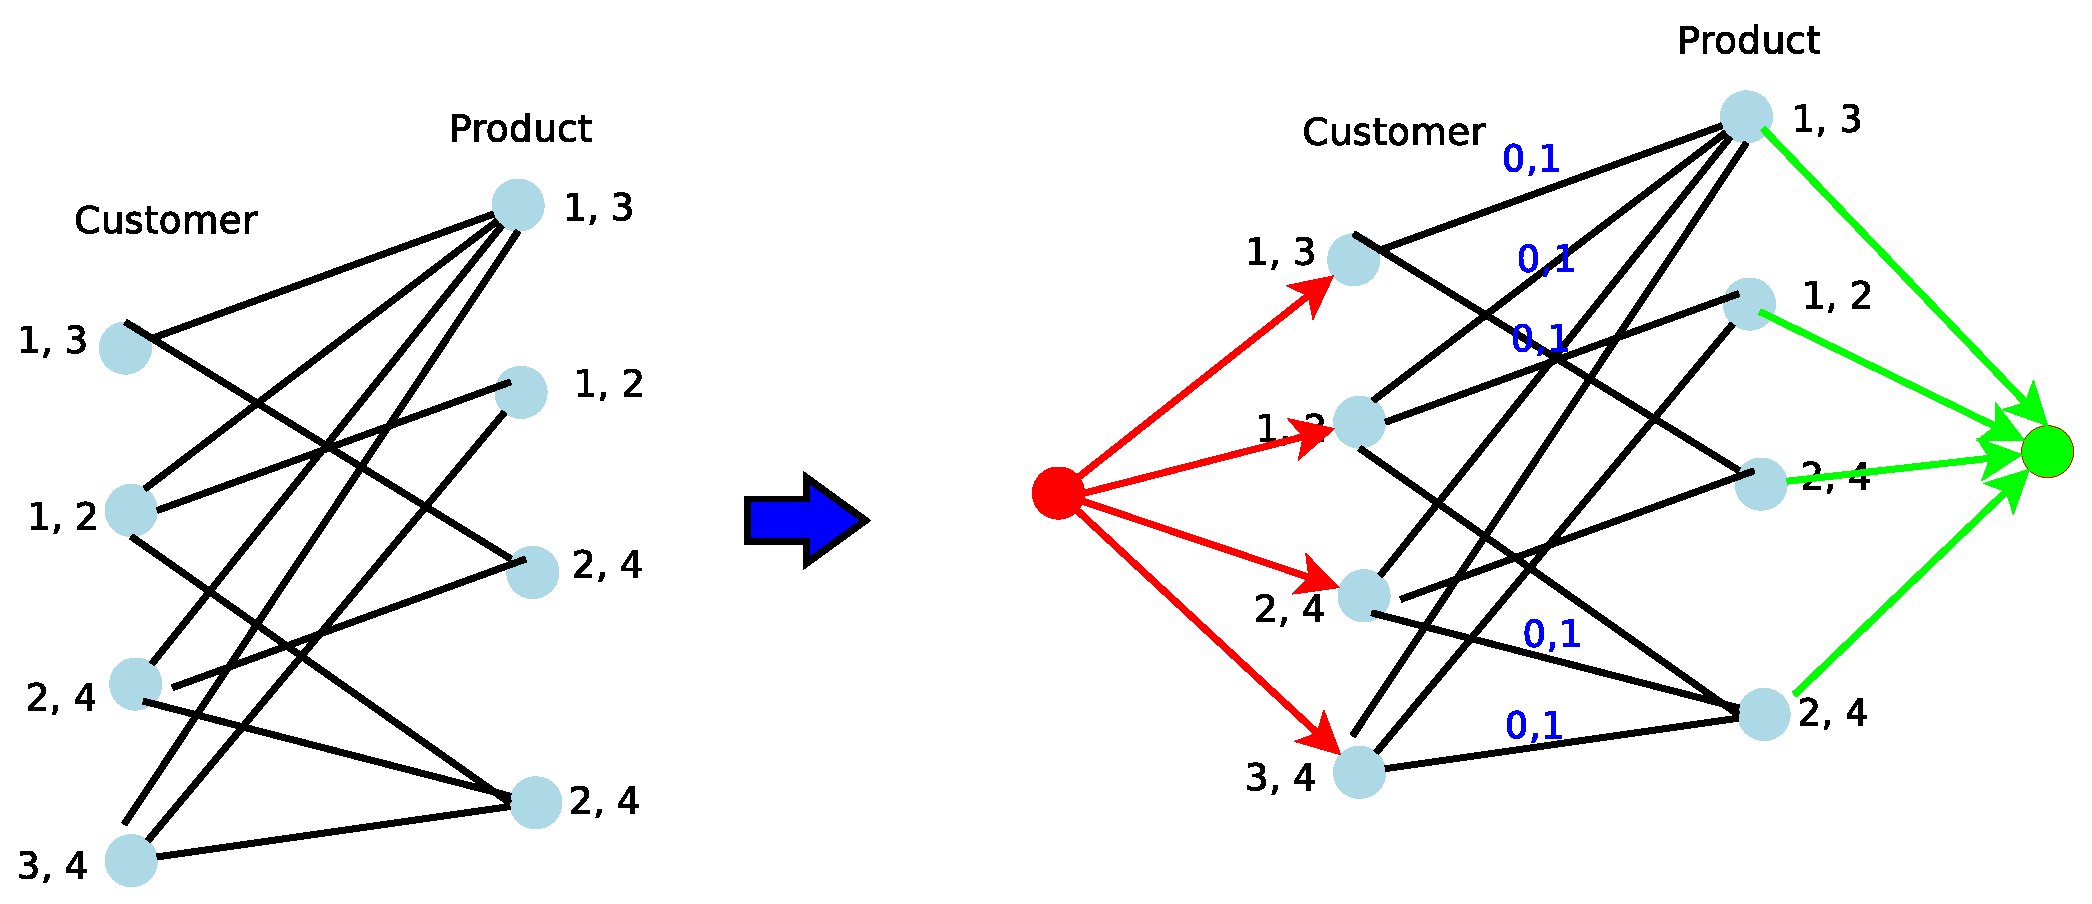
\includegraphics[width=4in]{L10-surveydesignexample-network.eps}
            \caption{将调查问卷设计问题转换为网络流问题}
            \label{Figure: survey_design_example_network}
        \end{figure}
        \paragraph{} 接下来我们建立这个问题对应的流网络:
        \begin{enumerate}
 \item 边: 引入两个节点$s$ and $t$. 将顾客连接到$s$并将产品连接到$t$.$s$点可以看所商场发信部门, 把问题发送到顾客, 而$t$点相当于商场的收件箱.
 \item 容量: 将节点上的权值移到边上; 并令中间这些边的权值均为$C(i,j)=1$;
 \item 流通: 一个原问题的可行解.
        \end{enumerate}
        \paragraph{}老样子, 这个问题也一样可以用线性规划求解, 我们这里就不多说了. 这个问题也很有用, 将来大家工作如果到商场电信部门, 估计就让大家干这事.
    \subsection{匹配}
        \subsubsection{二部图匹配}
        \paragraph{}我们首先来看最简单的二部图匹配:
        \paragraph{输入:} 二部图$G=<V,E>$;
        \paragraph{目标: } 找出最大匹配;
        \paragraph{}一个常用的比喻是: 如图\figurename\ref{Figure: matching_example}所示, 左边是男士, 右边是女士, 如果互相喜欢就连一条边, 如果不喜欢就不连边. 我们就相当于红娘, 问最多能成几对.
    \begin{figure}[h]
        \centering
        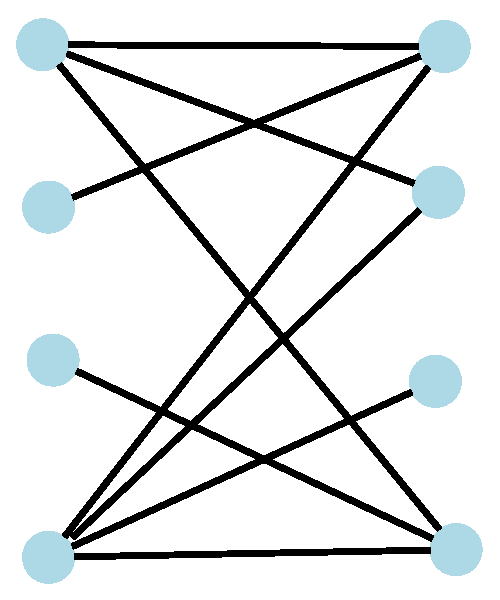
\includegraphics[width=1.in]{L10-matchingexample.eps}
        \caption{一个二部图匹配的例子}
        \label{Figure: matching_example}
    \end{figure}
    \paragraph{}对于这个问题, 我们有一比较简单的做法. 按如下方式建立流网络, 如\figurename\ref{Figure: matching_example_network}所示
    \begin{enumerate}
\item 边: 增加两个节点$s$和$t$; 将$s$连接到$U$并将$t$连接到$V$;
\item 容量: $C(e)=1, \forall e\in E$(这就保证了中间两排节点, 每个节点最多使用一次);
\item 流: 最大流对应于最大匹配;
\end{enumerate}
    \begin{figure}[h]
        \centering
        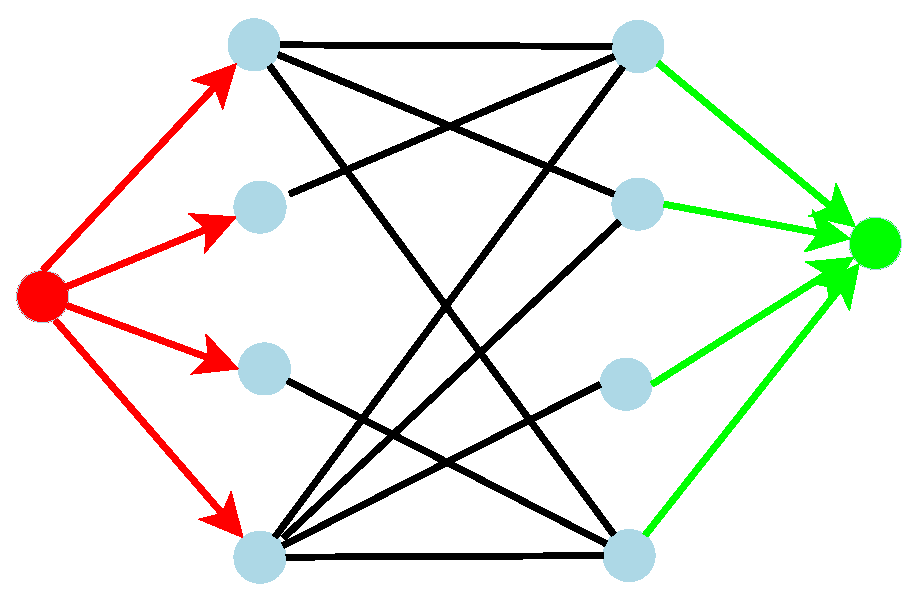
\includegraphics[width=1.5in]{L10-matchingexample-network.eps}
        \caption{二部图匹配问题对应的流网络}
        \label{Figure: matching_example_network}
    \end{figure}
    \paragraph{}算法时间复杂度为$O(mn)$
        \subsubsection{完美匹配}
        \paragraph{}上面我们已经解决了二部图上的最大匹配, 二部图上的匹配是很简单的. 但即便是对于二部图, 也有不是那么简单的东西: Hall在1935所给出的定理(Konig-Egervary在1931年给出). 我们首先给出完美匹配的定义(简单来讲就是所有人都有对象), 一个例子如\figurename\ref{Figure: matching_perfect_matching_example}所示.
        \begin{definition}[完美匹配]
给定一个二部图$G=<V,E>$, 其中$V=X\cup Y$, $X \cap Y = \phi$, $|X|=|Y|=n$. 一个匹配$M$是完美匹配当且仅当$|M|=n$.
        \end{definition}
        \begin{figure}[h]
            \centering
            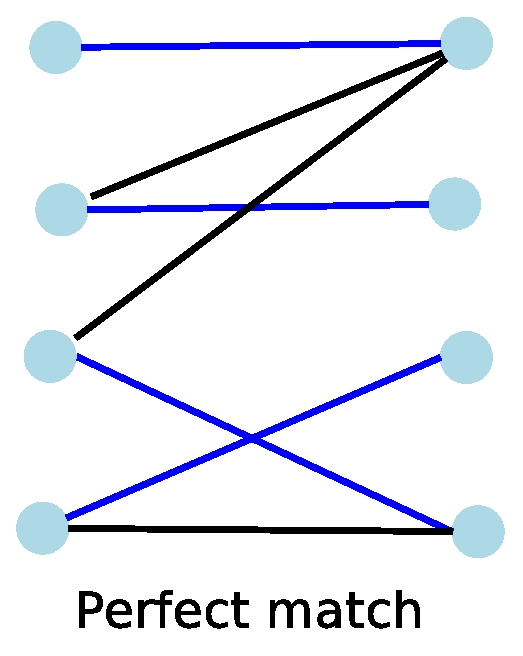
\includegraphics[width=1.in]{L10-perfectmatchingexample.eps}
            \caption{一个二部图完美匹配的例子}
            \label{Figure: matching_perfect_matching_example}
        \end{figure}
        
        
            \paragraph{}而这个定理如下所述, 这个定理不是很显然.
\begin{theorem}
一个二部图存在完美匹配 $\Leftrightarrow$ 对任意$A \subseteq X$, $ |\Gamma(A) | \geq |A|$, 其中$\Gamma(A)$表示$A$中匹配节点的集合.% denotes the partners of nodes in $A$.
\end{theorem}
            \paragraph{}用红娘的例子来说, 对一个如\figurename\ref{Figure: matching_perfect_matching_example}所示二部图, 假设左边是男士, 右边是女士, 每个人都有对象当且仅当: 任意挑一些男士(即$A$集合), 它们喜欢的女士(即$\Gamma(A)$)的数量大于等于这些男士的数量. 
            \paragraph{}这个定理反过来很好理解, 不如\figurename\ref{Figure: matching_perfect_and_imperfect_example}右边所示, 三维男士喜欢两位女士, 那肯定有一个人打光棍, 也就是不存在完美匹配. 正过来就不好理解了, 为什么所有集合的男士喜欢的女士比男士多的话就存在完美匹配? 所有男士的集合有$2^n$种, 不是那么好理解.

\begin{figure}[h]
        \centering
        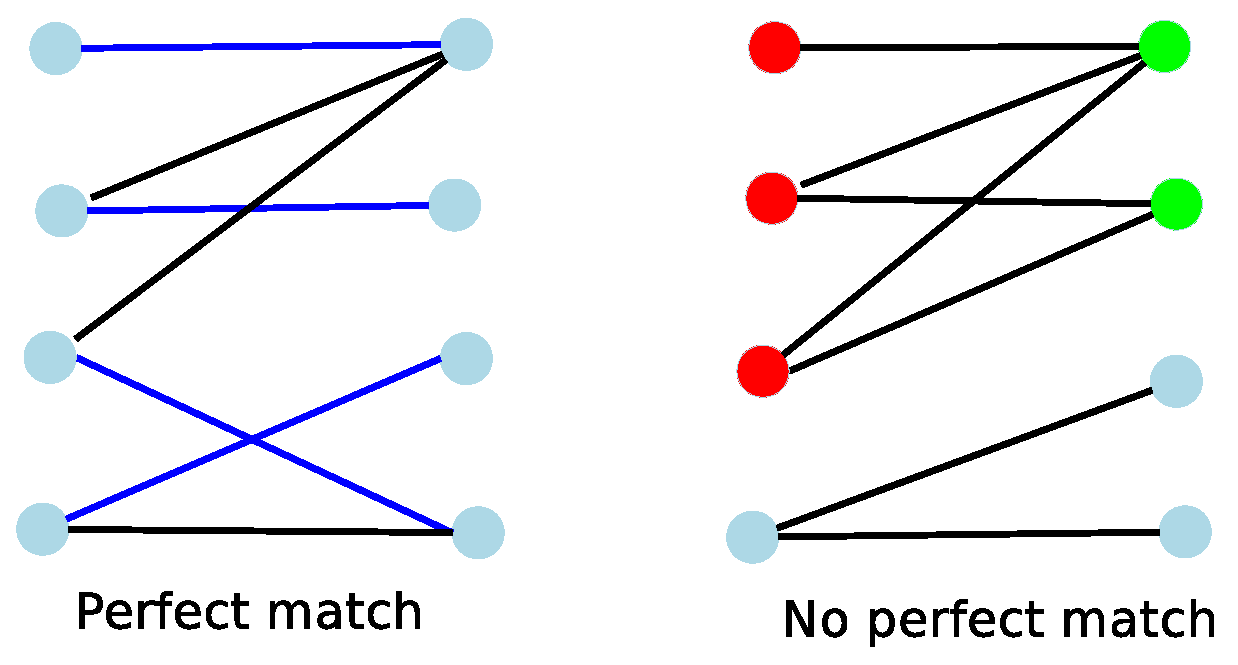
\includegraphics[width=2.2in]{L10-imperfectmatchingexample.eps}
        \caption{左侧的例子存在完美匹配, 而右侧的不存在完美匹配}
        \label{Figure: matching_perfect_and_imperfect_example}
\end{figure}
    
        \begin{proof}
我们只证明如果存在完美匹配, 那么$ |\Gamma(A) | < |A|$.
\begin{enumerate}
\item 假设不存在完美匹配, 也就是说, 最大匹配(成的对数)是$M$且$|M| < n$;
\item 我们考虑之前的流图, 考察它的最大流和最小割, 那么肯定存在一个割使得$C(A', B') < n$. 定义$A=A'\cap X$. 这个仅仅是把不存在完美匹配翻译成最大流的语言;
\item $C(A', B') = | X \cap B' | + | Y \cap A' | = n-|A| + | \Gamma( A ) |$, 如\figurename\ref{Figure: matching_imperfect_matching_example_proof}所示.
\item 因为$ C(A', B') < n$, 所以我们有$ |\Gamma(A) | < |A|$.
\end{enumerate}
\end{proof}
    \paragraph{}注意, 如果有必要, 我们可以改变$A'$使得$\Gamma(A)  \subseteq A'$. 这个算法时间复杂度为: $O(mn)$
        
        \begin{figure}[h]
            \centering
            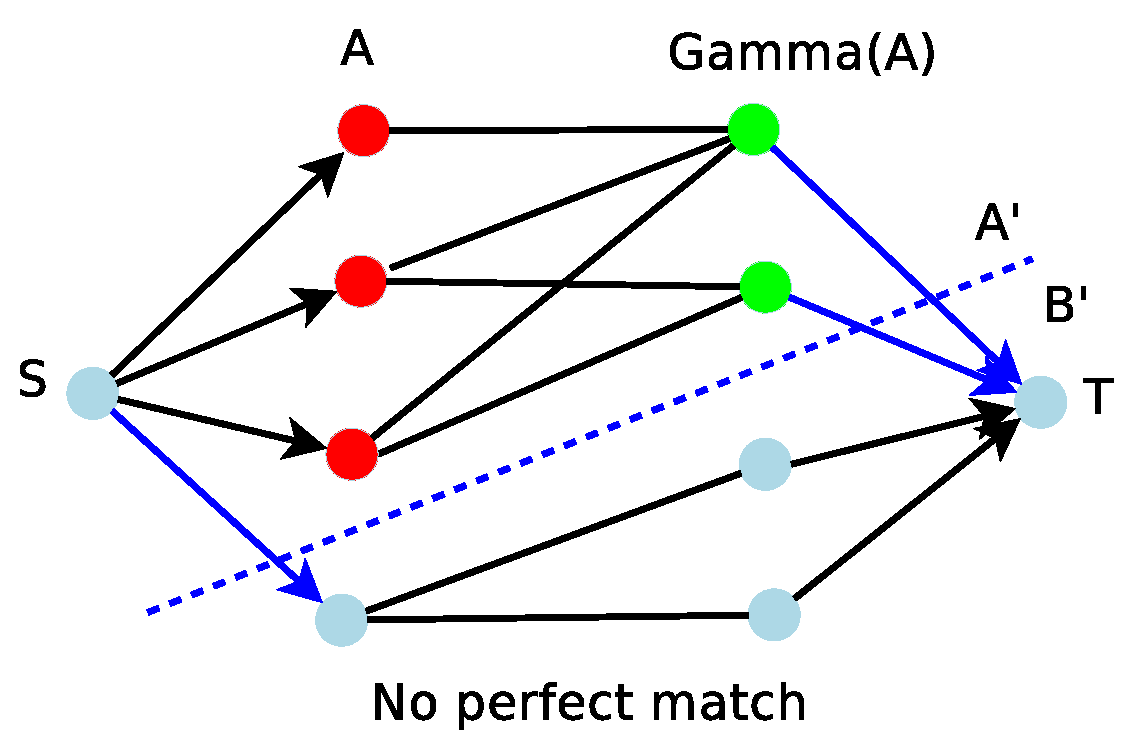
\includegraphics[width=1.8in]{L10-imperfectmatchingexampleproof.eps}
            \caption{\figurename\ref{Figure: matching_perfect_and_imperfect_example}中右图(不存在完美匹配)对应的网络图}
            \label{Figure: matching_imperfect_matching_example_proof}
        \end{figure}
        \paragraph{}也就是说, 这个定理告诉我们, 给了一堆喜欢的关系, 我们没有找到完美匹配, 原因就是其中几个人喜欢的人数太少了, 我们用上面的方法还能找到到底是哪些人. 这个定理很好理解, 但是它很深刻.


        \subsection{数字分解}
        \paragraph{}还有什么问题可以让我们想到最大流最小割呢? 把一个数字拆分. 一个应用是{\sc Baseball Elimination}问题. 不知道大家现在看不看足球, 有时当一个赛季快结束时, 有的球报上居然会出数学公式, 推算什么什么队(比如北京国安队)与冠军无缘. 定义如下:
        \paragraph{输入:}$n$个球队$T_1, T_2, ..., T_n$. 一个球队 $T_i$已经赢了$w_i$场球, 对$T_i$球队和$T_j$球队, 还有$g_{ij}$场球要踢.
        \paragraph{目标:}我们是否可以确定一支球队, 比方说$T_i$, 已经无法赢得冠军? 如果可以赢得冠军, 我们能给出证据吗?
%If yes, can we give an evidence?
        \paragraph{}下面我们给一个例子: 一共有4只球队: \textit{New York, Baltimore, Toronto, Boston}, 它们的$w_i$和$g_{ij}$如下:
        \begin{enumerate}
 \item $w_i$: 纽约 NY(90), 巴尔迪莫 Balt(88), 多伦多 Tor(87), 波士顿 Bos(79).
 \item $g_{ij}$: NY:Balt 1, NY:Tor 6, Balt:Tor 1, Balt:Bos 4, Tor:Bos 4, NY:Bos 4.
        \end{enumerate}
        \paragraph{}赛程过半, 我们就可以得到以上的数据, 这时我们已经可以肯定$Boston$已经无法取得冠军了, 因为一方面, $Boston$最多可以以$79+12=91$场胜利结束比赛(已经赢了的加上剩下的). 另一方面, 我们可以找到一个球队的子集(先不管怎么找的), 比如说$\{ NY, Tor \}$, 子集中球队结束时胜利的总数为$90+87+6 = 183$, 因此结束时至少有一支球队赢了$\frac{183}{2}=91.5 > 91$场球. 注意, 另一个子集$\{NY, Tor, Balt\}$就无法作为$Bos$已经无法取得冠军的证据.
        \paragraph{}我们可以把{\sc Baseball Elimination}问题形式化地表述如下:
        \paragraph{问题:} 对一个特定的球队$z$. 我们能否确定是否存在一个球队的子集$S \subseteq T-\{z\}$, 使得:
        \begin{enumerate}
 \item $z$可以以最多$m$场赢球结束所有比赛;
 \item $\frac{1}{|S|} ( \sum\nolimits_{x\in S} w_x + \sum\nolimits_{x,y\in S} g_{xy} )> m $;
        \end{enumerate}
        \paragraph{}换句话说, $S$集合中至少有一只球队赢场多余$z$.
        \paragraph{}我们以$z=Boston$为例来展示如何使用网络流解决这个问题. 首先, 我们令$m= w_z + \sum_{x\in T} g_{xz} = 91$, 也就是$z$球队可能赢的总场数. 接下来, 我们按如下的方式构造网络, 如\figurename\ref{Figure: matching_baseball_elimination_network}所示:
        \begin{enumerate}
 \item 令$S=T-\{z\}$且$g^*=\sum_{x,y\in S} g_{xy} = 1 + 6 + 1 = 8$.
 \item 节点: 对每两支球队, 构造一个节点${x:y}$(左边那三个点), 对每个球队$x$, 构造一个节点$x$(右边三个点).
 \item 边:
 	\begin{itemize}
 		\item $s$指向${x:y}$, 设置容量为$g_{x,y}$. 假设赢一场一分, 那么$s->$\{NY:Tor\}就相当于从$s$发射$6$分.
 		\item 连接$x:y-x$, 连接$x:y-y$, 容量都设为$g_{x,y}$. 对\{NY:Tor\}节点, 它们一共要踢$6$场(赢$6$分), 它一定要分解成\{NY:Tor\}到NY和\{NY:Tor\}到Tor.
 		\item 连接${x}-t$, 容量设为$m-{w_x}$. 比如NY到$t$的边, 纽约已经赢了$90$场了, 再赢$1$一场就比波士顿最多可能赢得要高了.
	\end{itemize}
        \end{enumerate}
        \begin{figure}[h]
            \centering
            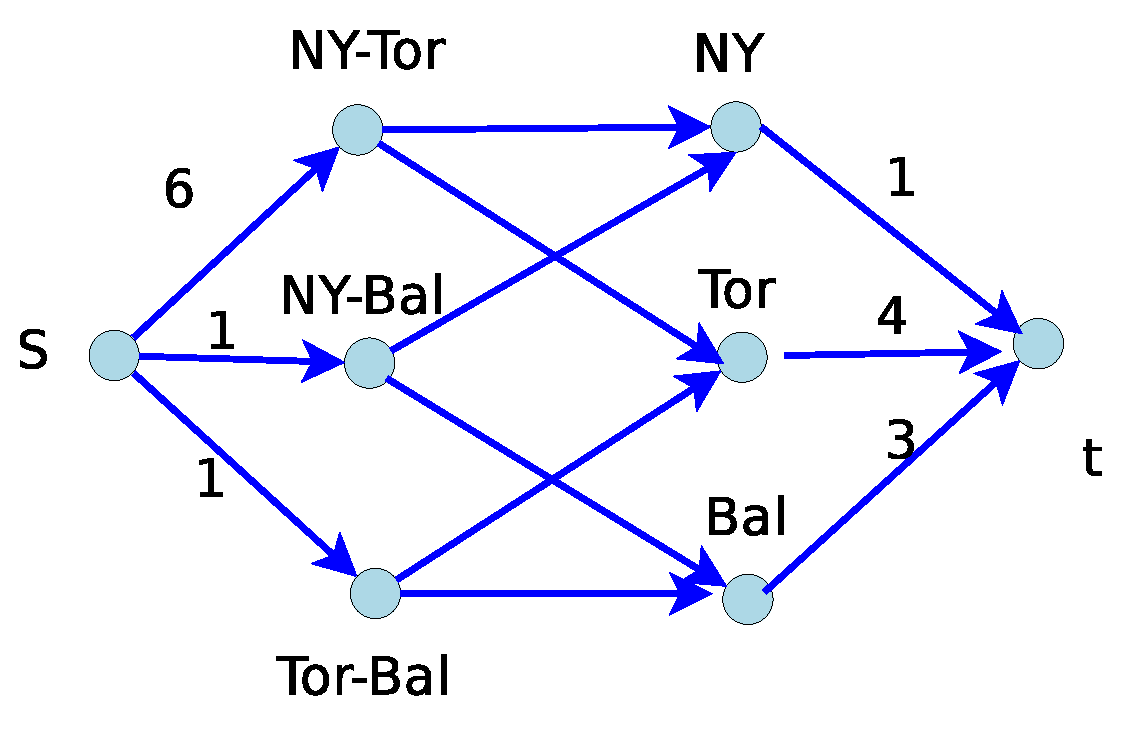
\includegraphics[width=1.9in]{L10-baseballelimination.eps}
            \caption{{\sc Baseball Elimination}问题的网络构造}
            \label{Figure: matching_baseball_elimination_network}
        \end{figure}
        
        \paragraph{}首先, 直觉上考虑, 沿着边$s-{x:y}$, 我们运送$g_{x,y}$次赢场. 在节点$x:y$, 这个数被分解成了两个数, 也就是两只球队的赢场. 这样, 这个问题就是一个数字分解问题.
         \paragraph{情况1:}最大流的值是$g*=8$ 

        \begin{theorem}
网络中存在一个值为$g^*=8$的流当且仅当球队$z=Boston$还有可能赢得冠军.
        \end{theorem}
        \begin{proof}
\begin{itemize} 
 \item $\Leftarrow$
如果有一个值为$g^*$的流, 那么边$x-t$上的容量保证了没有球队可以赢得超过$m$场球.因此, 球队$z$还有可能赢得冠军(只要$z$赢得剩下的所有比赛).
  \item $\Leftarrow$
如果球队$z$还有可能赢得冠军, 我们总可以找到一个值为$g^*$的流.
\end{itemize}
\end{proof}
        \paragraph{情况2:}最大流的值小于$g*=8$
        \begin{figure}[h]
            \centering
            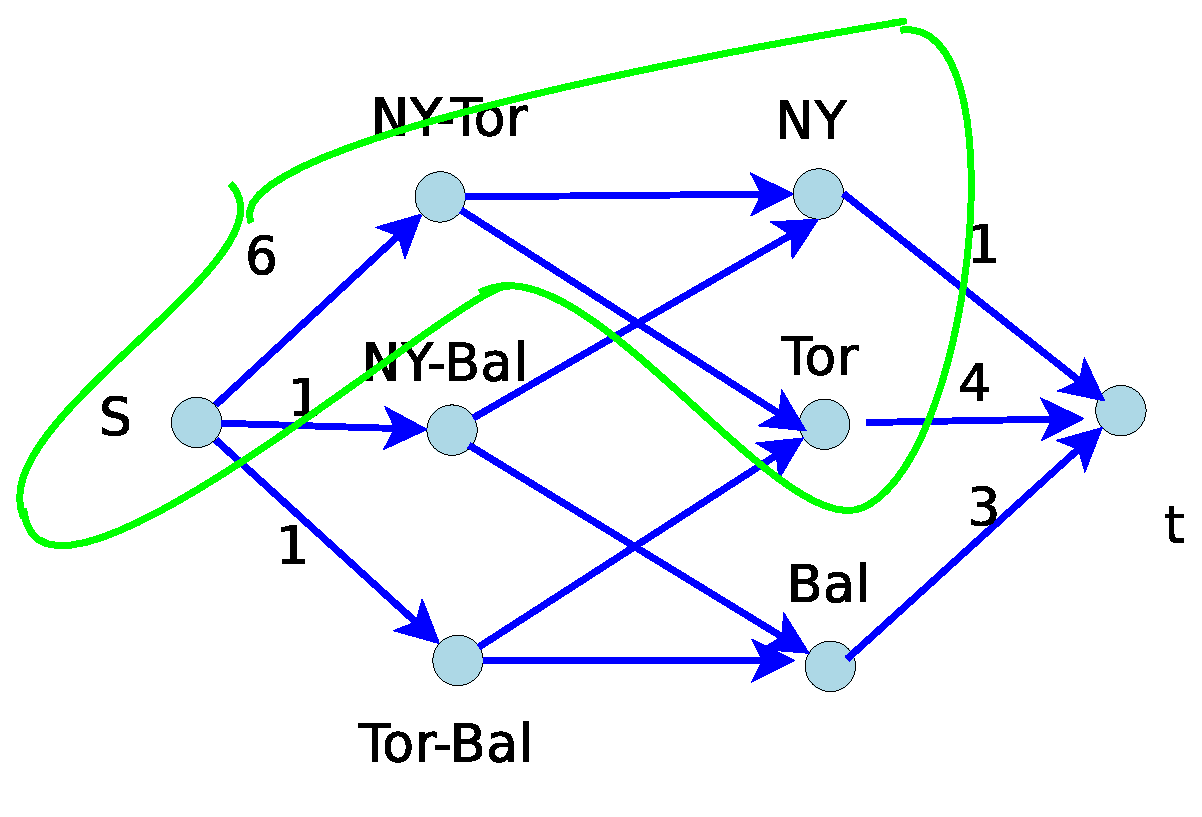
\includegraphics[width=2.in]{L10-baseballeliminationproof.eps}
            \caption{第二种情况}
            \label{Figure: matching_baseball_elimination_proof}
        \end{figure}
        \begin{theorem}
如果最大流值严格小于$g^*$, 最小割描述了一个子集$S \subseteq T-\{z\}$, 其使得$\frac{1}{|S|} ( \sum\nolimits_{x\in S} w_x + \sum\nolimits_{x,y\in S} g_{xy} ) > m$ \nonumber.
        \end{theorem}
        \begin{proof}
 (See extra slides)
        \end{proof}
        \paragraph{} 匹配问题还有很多扩展, 比如:指派({\sc Assignment})问题, 带权指派({\sc Weighted Assignment})问题的Hungarian算法, 开花(Blossom)算法.
        
 
 
 
%\end{document}